\part{Représenter et homogénéiser dans un format pivot XML TEI les métadonnées Lectaurep}\label{partie_2}

Nous venons de présenter les spécificités de la chaîne de traitement de Lectaurep qui fait circuler des ensembles de données structurées complexes qui sont manipulés et ne communiquent actuellement pas forcément entre-eux. Le premier objectif du DMC est de pouvoir récupérer les métadonnées de ces traitements spécifiques dans \textit{eScriptorium} et les associer à leurs informations déjà présentes en salle des inventaires virtuelles (SIV) pour enrichir et valoriser leurs fonds.

La première partie du stage comportait une réflexion sur la gestion et la création des métadonnées dans le cadre du projet Lectaurep et de la possibilité de les unifier au sein d'un même fichier. Cette mission s'est présentée sous la forme de questions : quelles métadonnées sont susceptibles d'être intégrées à la plate-forme eScriptorium lors de l'import des images ? Quelles métadonnées extraire une fois les traitements dans cette même plate-forme effectués ? Par ailleurs, quelles solutions pour modéliser et rendre interopérables les  métadonnées repérées ? Enfin, sur quel(s) référentiel(s) s'appuyer ?\footnote{LA première mission a été présentée sous la forme d'une \textit{issue} GitLab, URL : \url{:https://gitlab.inria.fr/almanach/lectaurep/documentation/-/issues/1} [à titre informatif, un accès peut être requis]}\\

Les réponses à apporter à ces questions ont nécessité plusieurs étapes de réflexion et la mise en place d'une stratégie dans l'application des technologies.\\

Dans un premier temps, une présentation de l'ensemble des métadonnées, de leurs référentiels associés ainsi que de leur circulation en terme de flux entrants et sortants dans la plate-forme eScriptorium, s'est avérée cruciale. En concertation avec l'ensemble des acteurs du projet, nous avons pu repérer un certain nombre de métadonnées à associer aux images lors des étapes d'import et d'export dans eScriptorium.\\

Dans un second temps, nous avons posé les avantages d'agréger ces données dans un fichier pivot XML répondant à la spécification TEI (\textit{Text Encoding Initiative}). Ce fichier doit permettre, à terme, d'échanger des ressources entre différents systèmes d'informations de Lectaurep. Il fut nécessaire de mettre en avant les atouts du modèle de la TEI, dans un contexte archivistique, en vue de la continuation du projet Lectaurep sur le long terme.\\ 

Une fois les définitions et les questionnements posés, nous avons pu préparer un environnement propice au développement \inquote{agile} de ce format pivot. L'intention était de garantir sa future évolution et d'expérimenter une première formalisation dans un fichier XML TEI (créé \textit{ex nihilo} pour l'occasion), avec un petit choix de métadonnées. Nous résumons ici ces différentes phases logiques.
\clearpage
\thispagestyle{empty}
\chapter{Enjeux et analyse des problématiques liées aux données Lectaurep et au format pivot XML-TEI}
\section{De l'importance de l'interopérabilité des données}
%\subsection{Données, métadonnées, interopérabilité et format pivot : définitions et objectifs pour Lectaurep}
\subsection{Définitions et objectifs de Lectaurep}
\subsubsection{Rappels généraux : données et formats}

Actuellement, la donnée est partout (\textit{data} en anglais) cependant son usage est trompeur et souvent mal compris. Elle n'est pas simplement quelque chose qui existe en soi, mais peut faire également l'objet d'une construction. Le terme de donnée renvoie à des contextes et des réalités différentes.\\

D'après le CNRTL, la \textbf{donnée} est ce qui est communément admis et qui sert de base à une recherche ou un raisonnement\footnote{\inquote{donnée}, CNRTL (Centre national des ressources textuelles et lexicales), URL : \url{https://www.cnrtl.fr/definition/academie8/donnée}}. D'après cette définition c'est donc une information codifiée, manipulable, transmissible et figée comme une mesure ou un fait observable. Ainsi la donnée brute ou primaire correspond à l'information tel qu'existe, par exemple un acte de notaire qu'un historien s'apprête à l'étudier.\\

En informatique, ces données manipulées sur un ordinateur sont de deux types. Dans un premier temps, les \textbf{données non structurées}. Ce sont celles qui existent sur un support informatique, mais qui n'ont pas fait l'objet d'une modélisation conceptuelle et ne sont pas stockées selon un format qui correspond à l'implémentation technique du modèle, comme par exemple du texte brut où les caractères sont représentés selon le standard UTF-8. Au contraire, les \textbf{données structurées} ont fait l'objet d'une conceptualisation durant laquelle on a pu déterminer pour ces données des propriétés et des champs de valeurs possibles; cette conceptualisation se traduit dans un format technique (l'information est codée). Une métadonnée est également une donnée structurée, dans le sens où elle est une donnée sur la donnée servant à décrire les caractéristiques d'une donnée brute en vue de faciliter son repérage, sa compréhension, sa gestion, son usage ou sa préservation selon les cas.\\

Dans la suite nous parlerons surtout de données structurées, nous utiliserons indistinctement les termes de données et de métadonnées pour qualifier la même chose.\\ 

Les données sont généralement représentées dans plusieurs types de formats au sein d'un \textbf{système d'information}\footnote{Un système d'information (SI) est un ensemble organisé de ressources (matérielles et logicielles) qui permettent de collecter, stocker, traiter et distribuer les données/métadonnées.} (SI) comme par exemple un tableau à double entrée, une base de données relationnelles ou un document XML. Le monde documentaire utilise principalement les formats basés sur les langages à balises reconnaissables grâce à leurs chevrons ouvrants et fermants (\citecode{< >}). Les plus connus sont ceux qui descendent du langage SGML\footnote{Le \textbf{SGML} ou \textit{Standard Generalized Markup Language} est un langage de description à balises. Apparu dans les années 1980, il a rendu possible l'exploitation des premières DTD (\textit{Document Type Definition}) qui est un schéma de déclaration des éléments utilisés selon des règles. Il est aujourd'hui abandonné au profit de ses descendants HTML, XHTML et XML apparus au moment de l'invention du \textit{web} dans les années 1990.} (\textit{Standard Generalized Markup Language}) et maintenus par le W3C\footnote{\url{https://www.w3.org}} (\textit{World Wide Web Consortium}). Par exemple, le HTML\footnote{Le \textbf{HTML} ou \textit{Hyper Text Markup language} est le langage de la page \textit{web} par excellence. Il sert à structurer sémantiquement du contenu et à rendre compte de son apparence. Cependant la mise en page du HTML est souvent réalisée avec le langage de programmation JavaScript (apparence dynamique) et du CSS (\textit{Cascading Style Sheets} pour l'apparence statique et dynamique de la page \textit{web}).} (\textit{Hyper Text Markup language}) qui permet de rendre compte d'une mise en page ou d'une typographie particulière d'un ensemble de données (texte stylisé ou \textit{fancy text}) pour les exposer le \textit{web}.\\

Omniprésent dans l'informatique documentaire, le balisage XML\footnote{Le \textbf{XML} ou \textit{Extensible Markup Language} est un langage de balisage extensible, héritier du SGML. Au même titre que son frère HTML, il est reconnaissable par l'usage de chevrons ouvrants et fermants : \citecode{< >}. Sa syntaxe est dite \inquote{extensible} car on peut définir ses propres noms de balises (grammaire). Les objectifs du XML sont l'encodage de ressources textuelles via son système de balises, l'échange de contenus complexes pouvant être représentés sous la forme d'arbres entre systèmes d'informations hétérogènes (intéropérabilité). Un document XML pour être \inquote{valide} doit respecter un schéma défini ou non par les utilisateurs (par exemple, une DTD ou un schéma RelaxNG) et posséder une syntaxe \inquote{conforme}. Ce qui est en fait un langage strict en dépit de son apparence d'\inquote{extensibilité}.} (\textit{Extensible Markup Language}) permet de décrire la logique et la sémantique des données. 

Un document XML respecte généralement des règles de syntaxe précises. Parmi les règles qui définissent un document XML \inquote{bien formé} ou \textit{well-formed} : les principes d'arborescences par imbrication d'éléments (l'élément enfant hérite des propriétés et attributs d'un élément parent) et non de recouvrement ; à chaque balise doit correspondre une balise de fin; il existe un seul élément racine (\textit{root element}) ; un élément ne peut posséder deux attributs du même nom. Les principes du langage XML sont résumés dans l'exemple ci-dessous : \\

\lstset{language=XML}
\begin{lstlisting}
<?xml version="1.0" encoding="utf-8"?> <!-- déclaration XML obligatoire -->
<elementParent couleur='rouge' position='milieuDroitePage'>
    <unElementEnfant id='1'>du texte</unElementEnfant>
    <unElementEnfant id='2'>encore du texte</unElementEnfant>
</elementParent>
\end{lstlisting} 
\newpage
Le format XML présente des avantages conséquents dans la représentation des données, il permet entre autre :
\begin{itemize}
    \item une bonne lisibilité par l'humain et la machine;
    \item une facilité d'intégration dans des plate-formes et logiciels;
    \item une migration vers d'autres formats;
    \item l'échange de données.
\end{itemize}


Toutefois, le format XML s'appuie généralement sur des spécifications qui décrivent des catégories d'objets en particulier. Ainsi une bibliothèque et un centre d'archives ne verrons pas de la même manière une archive et un livre en XML.\\

Les spécifications ou standards de représentation des données et des métadonnées répondent généralement à des normes techniques d'échange\footnote{Une \textbf{norme technique} est un référentiel publié par un organisme de normalisation officiellement agréé par l'État via une organisation nationale (comme AFNOR - Association française de normalisation ) ou internationale (comme ISO - Organisation internationale de normalisation). Le but étant d'harmoniser les pratiques d'un secteur d'activité suivant un cadre commun et de garantir un niveau d'ordre optimal.} de données et de métadonnées selon le contexte d'utilisation.\\

Les normes ISAD(G)\footnote{\textbf{ISAD(G)} (\textit{International Standard Archival Description-General}) ou Norme générale et internationale de description archivistique créé en 1994 sous l'impulsion du Conseil International des Archives (CIA, ICA en anglais) énonce les grands objectifs et principes de la descriptions archivistique et fourni une liste d'éléments de description que l'on peut employer dans un instrument de recherche, avec la définition de ces éléments et des exemples d'utilisation.} et ISAAR(CPF)\footnote{\textbf{ISAAR(CPF)} (\textit{International Standard Archival Authority Record for Corporate Bodies, Persons and Families}) ou Norme internationale sur les notices d'autorité archivistiques relatives aux collectivités, aux personnes et aux familles, est créé en 1995 par le Conseil International des Archives (ICA). La norme énonce les lignes directrices pour la description d'entités (collectivités, personnes, familles) associées à la production et à la gestion d'archives.} sont en vigueur dans le domaine archivistique pour décrire respectivement des fonds d'archives et des producteurs.

Dans le monde des bibliothèques, le catalogage repose également sur un ensemble de normes comme l'ISBD\footnote{\textbf{ISBD} (\textit{International Standard Bibliographic Description}) ou Description bibliographique internationale normalisée est une norme publié en 1971 et définie par l'IFLA (Fédération internationale des associations de bibliothécaires et d'institutions) pour la description du catalogage.} ou le \textit{Dublin Core} (norme ISO 15836) pour décrire des ressources bibliographiques.
\newpage
Dès lors il existe des implémentations de ces normes en XML. La norme ISAD(G) se trouve décliné en standard XML EAD\footnote{\textbf{EAD} (\textit{Encoded Archival Description}) ou description archivistique encodée, créé en 1993 et maintenue par la Bibliothèque du Congrès. S'appuyant sur la norme ISAD(G), l'EAD est utilisé pour décrire des fonds d'archives, des collections de manuscrits ou des collections hiérarchisés d'objets (photographies, numérisations, microfilms etc.), mais surtout pour encoder des instruments de recherche. L'ensemble des éléments XML sont présentés sur le site officiel : \url{https://www.loc.gov/ead/} et en français : \url{https://www.ead-bibliotheque.fr}} et ISAAR(CPF) en standard XML EAC-CPF\footnote{\textbf{EAC-CPF} (\textit{Encoded Archival Context - Corporate Bodies, Persons and Families}) s'appuie sur la norme définie par ISAAR(CPF) pour la rédaction des fiches de producteurs d'archives. C'est un schéma maintenu par la Bibliothèque d'État de Berlin et la SAA (\textit{Society of American Archivists}). Les éléments de l'EAC sont diponibles : \url{https://eac.staatsbibliothek-berlin.de}}.\\

Ces standards d'encodage sont généralement disponibles sous la forme d'un schéma de validation XML de type Relax NG\footnote{\textbf{Relax NG} (\textit{Regular Language for XML Next Generation}) est un langage de description de document XML permettant de définir les différentes contraintes qui déterminent l'imbrication des éléments ou la place des attributs dans le document pour passer l'étape de validation. C'est une puissante alternative au langage XML Schema.} ou DTD\footnote{\textbf{DTD} (\textit{Document Type Definition}) ou définition de type de document, est un document XML qui défini un modèle pour des fichiers XML et réglemente l'imbrication des balises, les noms d'éléments autorisés, la façon dont les attributs sont rattachés aux éléments. C'est un schéma XML moins sophistiqué que le Relax NG et XML Schema.} directement épinglé au document XML pour vérifier la strict validé de ce dernier. 
Si ces standards facilitent l'échange de certains type de données, ces dernières peuvent-elles communiquer entre elles ?\\

Nous verrons en détail dans la section \ref{Circonscrire un monde de données}, les formats et spécifications propres aux données et métadonnées qui nous ont particulièrement intéressés dans le cadre du projet.\\ 

\subsubsection{La question de l'interopérabilité dans Lectaurep}
Derrière ces définitions très généralistes, reposent des enjeux essentiels et concrets pour le projet Lectaurep et les utilisateurs de la plate-forme \textit{eScriptorium}. \\

Les répertoires de notaires numérisés qui sont importés dans la plate-forme \textit{eScriptorium} ne sont actuellement accompagnés d'aucune, sinon de très peu de métadonnées. Dès lors une annotatrice ou un annotateur qui travaille sur la transcription ou la segmentation d'une image, ne sera pas en capacité d'avoir des informations précises issues des instruments de recherche (producteur d'un document d'archives, cotes, informations techniques sur l'image). Un chercheur ou une chercheuse peut souhaiter des informations précises sur le fonds d'où est issue une transcription de répertoire.\\ 
\newpage
Lectaurep en tant que projet d'analyse et de reconnaissance de documents (ARD) est confronté au problème de la représentation des données pour couvrir des besoins utilisateurs diversifiés. Ainsi comme le souligne des chercheurs du LORIA (laboratoire lorrain de recherche en informatique et ses applications) et du laboratoire CNRS/ATILF de Nancy (Analyse et Traitement Informatique de la Langue Française) : 
\begin{quote}
    Il existe pour ainsi dire autant de formats de représentation des données que de systèmes de stockage ou de reconnaissance de document. Cette grande diversité est un frein certain à l'échange des données d'un environnement à un autre, d'une plate-forme à une autre et rend souvent les sorties de certains systèmes utilisables uniquement par eux-mêmes.\footnote{\cite{belaid_representation_2007}, pp.1-2}
\end{quote}

Le premier objectif pour Lectaurep est donc celui de l'\textbf{interopérabilité}\footnote{On parle généralement du principe ou de l'objectif FAIR (Facile à trouver, Accessible, Interopérable, Réutilisable) dans une plate-forme pour évoquer le fait que les données doivent être échangeables et identifiables pour permettre des bonnes performances.} des données et des métadonnées dans \textit{eScriptorium}. Soit la capacité de faire communiquer les données et métadonnées entre-elles, de les relier. Les données et métadonnées susceptibles d'être importées dans \textit{eScriptorium} suivent pour l'heure des modèles différents.\\

La plate-forme \textit{eScriptorium} ne prend, actuellement, en charge que des imports d'images au format .jpg ou .jpeg via une fonctionnalité de type \inquote{Glisser/Déposer} (\textit{Drag \& Drop}) ou avec l'URI\footnote{\textbf{URI} (\textit{Uniform Resource Identifier}) ou identifiant uniforme de ressource est une chaîne de caractère identifiant une ressource dans un réseau répondant à une norme du W3C pour le \textit{web} (Cf. RFC 3986). Une URL (\textit{Uniform Resource Locator}) comme par exemple \inquote{http://www.lectaurep.fr/} est un type d'URI qui identifie la ressource (la page de lectaurep), qui implique la représentation de la ressource en HTML obtenue via le protocole HTTP (\textit{Hypertext Transfer Protocol}, principal protocole de communication client-serveur dans le \textit{web}).} du manifeste IIIF et les transcriptions dans les formats XML ALTO\footnote{\textbf{ALTO} (\textit{Analysed Layout and Text Object}) est un standard XML rendant compte de la mise en page physique et de la structure logique d'un texte transcrit par reconnaissance optique de caractère (OCR/HTR). On y retrouve les coordonnées de segmentation (\textit{baseline}, polygones etc.), des éléments de forme (type de police etc.), ou encore des métriques (taux de confiance de reconnaissance). Le schéma de ce standard est maintenu par la Bibliothèque du Congrès et la BnF. \url{https://www.loc.gov/standards/alto/}}, XML PAGE\footnote{\textbf{PAGE XML} est le principal format de données utilisé par le logiciel Transkribus, il agrège l'ensemble des données relatives à l'image transcrite, le texte transcrit, les coordonnées de zones de texte, les corrections effectuées etc. Pour comprendre les différences entre le XML ALTO et le XML PAGE on pourra se rapporter à \cite{bonhomme_defis_2018}, pp. 46-47. Le schéma est disponible : \url{https://www.primaresearch.org/schema/PAGE/gts/pagecontent/2016-07-15/pagecontent.xsd}}, pour les utilisateurs qui souhaiteraient reprendre leurs travaux de transcription en cours. Lors de l'export, on peut récupérer le résultat de sa transcription (pour la sauvegarde notamment) au format XML ALTO ou XML PAGE, ou encore simplement en texte brut.\\

Dès lors, on retrouve un format de fichier par type de données, certains formats étant mieux adaptés pour contenir et décrire certains types de données que d'autres. En revanche, cela présente le désavantage, pour les utilisateurs, de ne pas avoir accès à l'ensemble des données et des métadonnées lors de l'import/export de leurs travaux dans la plate-forme.\\

Les utilisateurs devraient pouvoir récupérer à la fois l'image de la numérisation du répertoire de notaires, sous la forme d'une URI IIIF ou encore d'un chemin vers une ressource stockée localement, le résultat de sa transcription (vérité terrain ou résultat HTR), des métadonnées sur l'archive (producteurs, date, étude de notaire ou autre), provenant des instruments de recherche du DMC, l'historique de ses traitements (binarisation, segmentation, transcription etc.), et tout cela en une seule fois, lors de l'import et de l'export dans eScriptorium.    

\subsubsection{Une solution, le format pivot XML}
La figure \ref{fig:modèle_métadonnées_vise_V4} représente le modèle hypothétique envisagé par Lectaurep pour l'utilisation du format pivot et de ses usages à terme dans eScriptorium. \\
\begin{figure}[h]
    \centering
    \centerline{\fbox{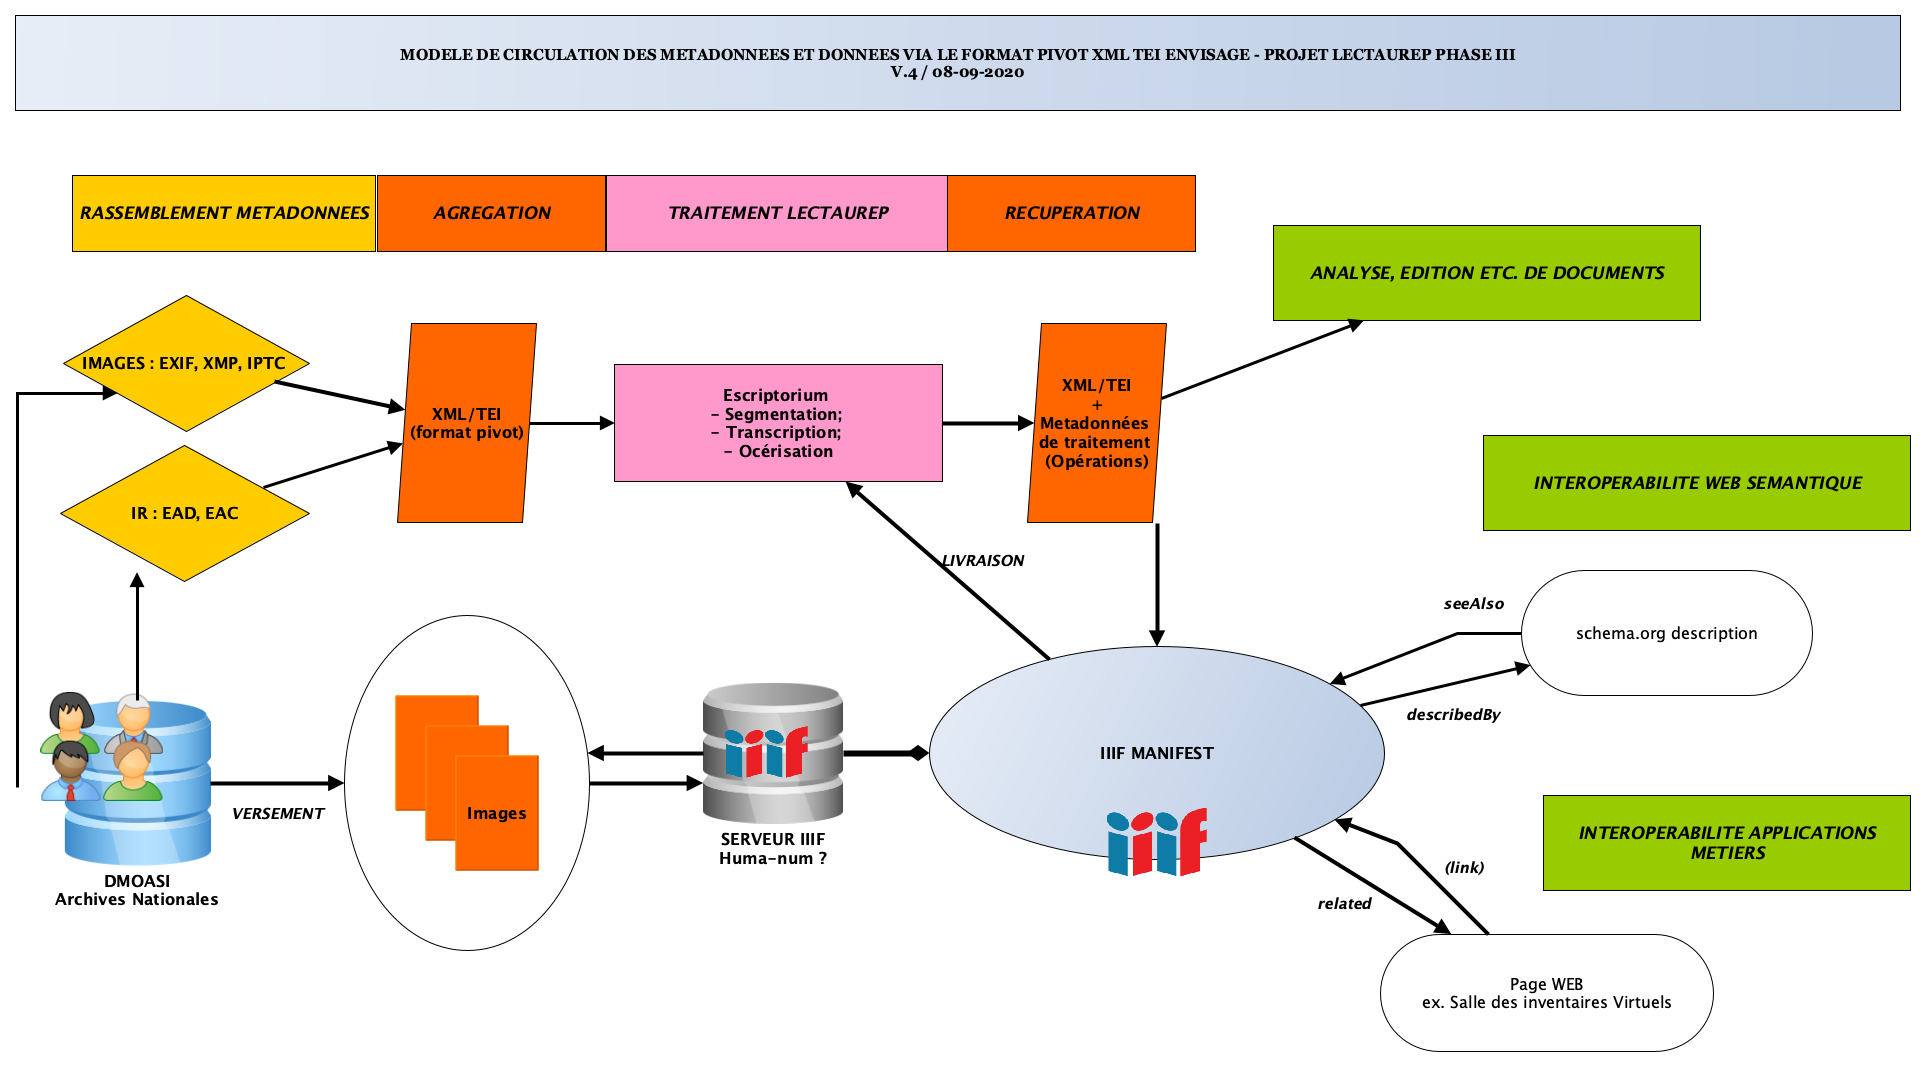
\includegraphics[width=18cm]{modèle_metadonnées_vise_V4}}}
    \caption{Schématisation du modèle de circulation des données dans eScriptorium souhaité par Lectaurep à terme  \textcopyright L. Terriel, 2020, yEd}
    \label{fig:modèle_métadonnées_vise_V4}
\end{figure}

Avant d'aborder la TEI comme modèle de données, le format pivot XML est la solution qui a été envisagé pour permettre une intéropérabilité des spécifications des données Lectaurep dans \textit{eScriptorium} durant mon stage. Il représente un bon point de départ pour traiter et agréger des flux entrants et sortants de données et des métadonnées dans une application. Cependant, pour être opérationnel et intégrable, le format pivot doit répondre aux critères\footnote{Ces critères d'évaluation du format pivot sont adaptés de l'article \cite{crozat_standardisation_2006}} de : 

\begin{itemize}
    \item \inquote{délimitation} : simple à utiliser pour n'importe quel type d'applications, les données et métadonnées utilisées doivent être identifiables dans ce format;
    \item \inquote{soutenance} : intégrer à un environnement technique permettant son évolution (modification), son implémentation facile et sa documentation;
    \item \inquote{spécification} : chaque projet répond à des caractéristiques originales qui lui sont propres, cependant l'appui sur un schéma déjà existant et ouvert (modulable) permet de créer une ligne directrice, pour un développement rapide.
\end{itemize}

Nous verrons que si le format pivot peut sembler indéniable pour faire converger des données de différents SI dans Lectaurep, le choix du modèle de représentation des données Lectaurep dans ce format pivot s'avère en revanche moins évident à définir (Cf. parties \ref{negatif_TEI} et \ref{positif_TEI}). 

\subsection{\inquote{Circonscrire un monde}, un focus sur les données de Lectaurep}\label{Circonscrire un monde de données}

Avant de concevoir la mise en place d'un fichier pivot XML, il faut comprendre quels sont les types de données que l'on va y intégrer. Nous pouvons décrire cette étape comme \inquote{circonscrire le monde}\footnote{\cite{poupeau_visite_2019}} des données et des métadonnées de Lectaurep. Ainsi j'ai effectué un premier travail de repérage durant le stage sur l'ensemble des données et métadonnées circulant dans les SI rattachés à Lectaurep. Ils sont donc susceptibles d'être récupérés lors des phases d'import ou d'export des images dans eScriptorium, dans le fichier pivot XML.
La figure \ref{fig:modélisation_données_lectaurep} montrent ces données, leur circulation et leurs relations en terme de SI. Nous avons cherché à brosser le tableau des métadonnées et des données de Lectaurep de la manière suivante :\\

\begin{figure}[H]
    \centering
    \centerline{\fbox{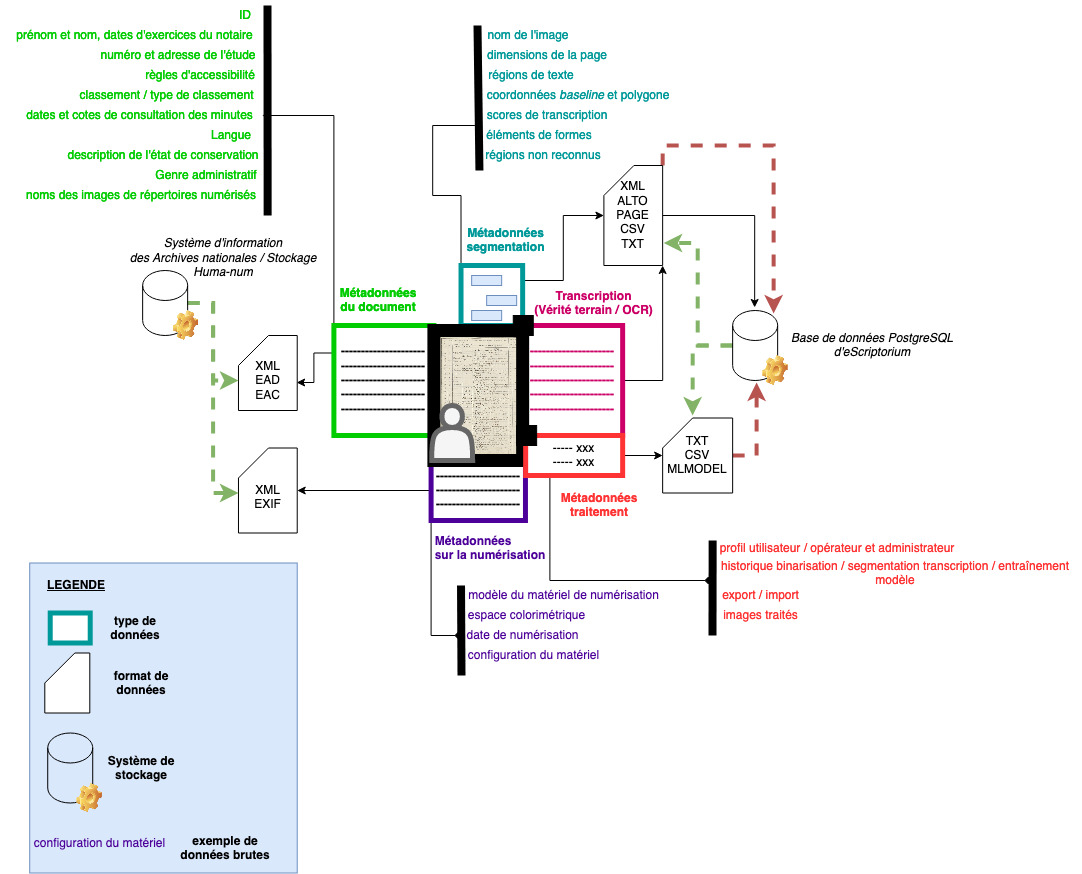
\includegraphics[width=15cm]{modélisation_données_lectaurep}}}
    \caption{Modélisation conceptuel des données, des formats et des systèmes d'informations du projet Lectaurep \textcopyright L. Terriel, 2020, Diagrams.net}
    \label{fig:modélisation_données_lectaurep}
\end{figure}

\textbf{Informations relatives aux répertoires de notaires en tant que documents d'archive -} Il s'agit des informations contenues dans les instruments de recherche\footnote{Un \textbf{instrument de recherche} est un outil papier ou informatisé énumérant ou décrivant un ensemble de documents d'archives de manière à les faire connaître aux lecteurs, définition issue de \cite{noauthor_abrege_2020}} (IR) en XML EAD et les notices producteurs (NP) 
en XML EAC-CPF\footnote{Pour consulter des exemples de ces fichiers Cf. Annexes, \citecode{/B-Format\_pivot\_XML\_TEI\_Lectaurep/Generator\_Lectaurep2TEI/Sets\_test\_Legay/Data\_xml\_ead\_eac/}}.
Ils sont récupérables dans la Salle des inventaires virtuels (SIV) dépendant du SI des AN\footnote{\url{https://www.siv.archives-nationales.culture.gouv.fr/siv/cms/content/display.action?uuid=Accueil1RootUuid&onglet=1}} et parfois sur le \textit{ShareDocs} dédié au projet.\\

Le DMC disposent de deux types d'IR par notaire tel que :
\begin{itemize}
    \item un instrument de recherche sous la forme \inquote{Minutes et répertoires du notaire 
    $M^{e}$N} : il s'agit d'un inventaire des actes, accompagné de descriptions détaillées de chacune des minutes de notaires et des répertoires eux-même;
    \item un instrument de recherche sous la forme \inquote{Images des répertoires du notaire $M^{e}$N} : il s'agit d'un inventaire spécifique les images numériques du répertoire d'un notaire donné.
\end{itemize}
Ainsi que deux types de NP par notaire tel que :
\begin{itemize}
    \item une notice producteur spécifique à l'étude du notaire;
    \item une notice producteur spécifique au notaire lui-même.
\end{itemize}
Ces fichiers contiennent généralement des métadonnées administratives pour la gestion (identification des archives, provenance et contexte de production de ces archives, intégrité, droits, etc.) et des métadonnées descriptives telles que les nom et prénom du notaire, le numéro de l'étude, l'adresse, le type de répertoires ou autre. \\

Ces  métadonnées sont reliées à la donnée brute, le répertoire en tant qu'archive matérielle, et à la copie numérique de celui-ci, son image. Dès lors, il existe entre ces différents IR et les NP des liens et des informations redondantes. Il est alors possible de faire en sorte de les croiser dans le fichier pivot XML, à l'image du numéro de l'étude, du nom du notaire, la cote du répertoire, les dates extrêmes d'exercice du notaire par exemple.\\

\textbf{Informations techniques relatives aux images numérisées de répertoires de notaires -} Ces métadonnées sont généralement contenues dans les images des répertoires numérisés. Les images sont pour l'instant disponibles sur le \textit{ShareDocs} dédié au projet. À terme, Lectaurep à pour ambition de disposer d'un serveur IIIF dédié au stockage des images et à la récupération de celles-ci, notamment par l'intermédiaire d'URI stables. L'avantage de ce stockage repose sur le fait qu'\textit{eScriptorium} peut consommer des images IIIF à partir de ces URI sans avoir à les charger ou à les dupliquer.\\

Les métadonnées techniques des images, qui ont intéressé le DMC durant mon stage, correspondent aux informations sur la numérisation des images et sont exposées au format EXIF \footnote{\textbf{EXIF} ou \textit{Exchangeable image file format} est une spécification de format de fichier pour les images utilisés par les appareils photographiques numériques ou les appareils de numérisation. Cette spécification repose sur des formats existants tels que le JPEG, JPG, TIFF (mais pas le JPEG 2000 ni le PNG. Pour accéder aux principaux champs EXIF et à leurs descriptions : \url{https://exiftool.org/TagNames/EXIF.html}} (\textit{Exchangeable image file format}). Pour y avoir accès, on utilise un logiciel de traitement d'images de type \textit{GIMP} ou \textit{XnView} ou par le biais d'un script Python utilisant le package \textit{PyExifTool} (Cf. Figure \ref{fig:sortie_exif_metadata}). 

\begin{figure}[h]
\lstset{language=Python}
\begin{lstlisting}
EXIF:ImageDescription => 74 - Main frame
EXIF:Make => i2S, Corp.
EXIF:Model => SupraScanII [SN: 283910] - Cam7600RGB [SN: 283910]
EXIF:Orientation => 1
EXIF:XResolution => 300
EXIF:YResolution => 300
EXIF:ResolutionUnit => 2
EXIF:ModifyDate => 2015:09:07 09:45:39
EXIF:YCbCrPositioning => 1
EXIF:ExifVersion => 0230
EXIF:CreateDate => 2015:09:07 09:45:39
EXIF:ComponentsConfiguration => 1 2 3 0
EXIF:FlashpixVersion => 0100
EXIF:ColorSpace => 65535
\end{lstlisting}
\caption{Un exemple de métadonnées EXIF extraites d'une image de répertoire numérisée et affichées en sortie d'un script Python utilisant le module \textit{PyExifTool}  \textcopyright L. Terriel, 2020, \textit{Pycharm}}
\label{fig:sortie_exif_metadata}
\end{figure}
\newpage
Enfin , il est possible d'exposer les données répondant à la spécification EXIF dans un format XML à condition d'utiliser le bon espace de nom sur les balises et le bon schéma XML associé.\\

\textbf{Informations liées à la transcription des vérités terrains et HTR des répertoires de notaires -} 
Les agents des AN rattachés à Lectaurep réalisent actuellement dans la plate-forme eScriptorium des transcriptions à partir des images de répertoires dans le but d'éditer des vérités terrains afin d'entraîner des modèles de segmentation. Ces données peuvent être importées ou exportées dans des fichiers XML ALTO, XML PAGE ou encore en texte brut. À terme, la transcription réalisée automatiquement par le modèle HTR dans \textit{eScriptorium} sera exportée dans ces types de fichiers. Pour prendre le cas des XML ALTO\footnote{Pour consulter des exemples de ces fichiers Cf. Annexes, \citecode{/B-Format\_pivot\_XML\_TEI\_Lectaurep/Generator\_Lectaurep2TEI/Sets\_test\_Legay/Data\_xml\_alto/}} (format privilégié pour l'export des transcriptions de vérité terrain), on y retrouve parfois des informations relatives à la mise en page physique, à l'emplacement d'une zone texte et d'une ligne de base sous la forme de coordonnées : zones de textes (paragraphe et polygones) et ligne de base du texte \textit{baseline} ainsi que le texte transcrit par l'utilisateur ou l'utilisatrice d'\textit{eScriptorium}.\\

\textbf{Informations liées à l'historique des traitements dans la plate-forme eScriptorium -} \textit{eScriptorium} conserve la trace des transactions  : informations sur le compte de l'usager, historique des traitements (segmentation, binarisation, transcription, etc.) et des opérations d'import et export. Ces données sont stockées dans le \textit{back-office} de l'application, dans une base de données SQL\footnote{\textbf{SQL} (\textit{Structured Query Language}) ou langage de requête structuré, est un langage informatique servant à exploiter des bases de données relationnelles. Il permet principalement de rechercher (\citecode{SELECT}), d'ajouter (\citecode{INSERT}), de supprimer (\citecode{DELETE}), ou de modifier (\citecode{UPDATE}) des données dans la base constituée.} de type \textit{PostgreSQL}\footnote{PostgreSQL est un type de système de gestion de base de données relationnelle et objet (SGBDRO).}. Certaines de ces données\footnote{On peut avoir un aperçu des migrations de données opérées lors des transactions dans l'interface en parcourant les scripts Python de l'application eScriptorium, \url{https://gitlab.inria.fr/scripta/escriptorium/-/tree/master/app/apps}} devront à terme  être intégrées dans le fichier pivot XML de Lectaurep à l'import et à l'export des images dans eScriptorium.\\

Nous avons déjà souligné, la notion selon laquelle l'encodage de ces données en XML constituait un dénominateur commun, exception faite pour la dernière catégorie évoquée précédemment, accessible par l'intermédiaire du langage SQL. Les parties qui vont suivre, proposent de mettre en avant les avantages qu'offre une modélisation TEI des données Lectaurep. Durant ce stage, nous avons choisi de nous concentrer sur un choix restreint de données et de métadonnées. Elles proviennent des catégories évoquées plus haut, et permettent de constituer une première représentation du fichier pivot XML TEI de Lectaurep, ce sur quoi nous reviendrons également par la suite. 

\section{Le format pivot XML TEI, un choix réaliste ?}
\subsection{La TEI pour annoter les données et les métadonnées de Lectaurep}

La \textit{Text Encoding Initiative}\footnote{Pour de plus de détails sur l'histoire, le fonctionnement et les usages de la TEI consulter \cite{burnard_quest-ce_2015}} (TEI) est sans doute l'un des plus importants projets d'application de l'informatique au domaine des sciences humaines et sociales. Dans \inquote{40 ans de relations entre les sciences humaines et informatique}\footnote{Lou Burnard, \inquote{Du \textit{literary and linguistic computing} aux \textit{digital humanities} : retour sur 40 ans de relations entre sciences humaines et informatiques}, in \cite{mounier_dir_readwrite_2012}}, Lou Burnard, chercheur de l'Université d'Oxford et cofondateur de la TEI, fait remonter l'apparition du projet TEI au deuxième âge des humanités numériques situé au début des années 1980.  Après une période qu'il intitule \inquote{\textit{Litterary and linguistic Computing}} marqué par les techniques statistiques de l'histoire quantitative, la TEI émerge dans la période des \inquote{\textit{Humanities Computing}}. Le chercheur s'éloigne alors du paradigme quantitatif (sans réellement le quitter\footnote{En 1983, la revue \textit{Histoire \& Mesure} parrait en France.}), pour encoder et structuré des informations qu'il parait utile de conserver et d'exploiter.

La TEI, créée en 1987, vise à standardiser les pratiques d'encodage et de structuration des textes chez les chercheurs. Mise en pratique dans un premier temps dans le cadre du langage SGML, elle devient ensuite une norme d'encodage pour le langage XML, applicable, en principe, à n'importe quelle source textuelle numérisée. L'outil est structuré autour d'une communauté pluridisciplinaire, composée d'historiens, de linguistes, de philologues ou encore d'archéologues. Ces professions utilisent et adaptent cette norme selon leurs besoins tout en suivant les recommandations de l'un des 21 modules d'éléments décrits dans les \textit{guidelines TEI P5}\footnote{Les \textit{guidelines TEI P5}, manuels, tutoriels, outils pour l'encodage de texte sont accessibles à l'adresse : \url{https://tei-c.org/guidelines/P5/}}.\\

Il s'agit d'une avancée considérable, évitant la sédimentation ou la \inquote{babélisation} numérique, où chacun proposerait son propre langage d'encodage suivant sa propre théorie. Ce \inquote{métalangage} commun offre un cadre de travail et une structure assez souple pour pouvoir s'adapter à chaque projet ou discipline.\\

Ce dispositif commun permet en particulier, une intéropérabilité minimale entre les données, objectif apprécié et recherché dans le projet Lectaurep. Au travers de la norme TEI, il sera possible d'encoder les informations des différents SI de l'éco-système Lectaurep (présenté dans la partie 3.1.2) dans un format qui permet leur structuration, leur alignement (au moyen de liens entre celles-ci), leur diffusion (vers d'autres formats de données ou d'autres programmes, par exemple) et leur archivage à long-terme, mais aussi, comme nous l'évoquions en section \ref{potentialités_TAL}, d'annoter des informations plus spécifiques comme les entités nommées issues des traitements du TAL. 

\subsection{Faire converger les standards de données vers un fichier pivot XML-TEI : confronter des visions opposées sur le document...}\label{negatif_TEI}

Lors d'un colloque organisé, en 2019, aux Archives diplomatiques de La Courneuve, le chercheur en humanités numériques Seth Van Hooland rappelait en substance que \inquote{les standards de métadonnées et les ontologies sont comme les sous-vêtements, tout le monde est d'accord sur le fait qu'ils sont nécessaires, mais personne ne veut utiliser le standard de quelqu'un d'autre.}\footnote{\cite{hooland_application_2019} on retrouve également 
une seconde version de cette anecdote dans \cite{gillet_introduction_2016}, pp.102.}. Derrière le caractère humoristique et anecdotique de la formule, le chercheur expose une réalité certaine pour les institutions patrimoniales : un musée, une bibliothèque, un centre d'archives et même les institutions de recherches, portent des regards très différents sur les documents. Les spécifications sont rattachées à des usages métiers ancrés dans le temps.\\

Durant le stage, ce fut une dimension à ne pas minimiser lors des réunions,  engageant un dialogue constant entre les ingénieur(e)s et les archivistes du projet Lectaurep sur les atouts de la TEI pour Lectaurep. Les principaux reproches qui peuvent être fait à la TEI sont souvent basés sur des comparaisons avec la grammaire EAD et peuvent être en partie résumés ainsi :\\
\begin{itemize}
    \item La philosophie de la TEI peut être éloignée des spécifications habituellement utilisées dans le monde documentaire tel que l'EAD. Dominique Stutzmann, chercheur du laboratoire IRHT\footnote{Institut de recherche et d'histoire des textes} du CNRS, note à ce propos : 
    \begin{quote}
        Les deux formats ont une philosophie différente. L'un est fait pour \inquote{enrichir} du \inquote{texte} 
        (\textit{Text Encoding Initiative}) et l'autre pour \inquote{décrire} des \inquote{archives} (je triche un peu, ici, puisque le mot \textit{encoded} se trouve aussi dans \textit{Encoded Archival Description})\footnote{\cite{stutzmann_ead-tei_2019}}.
    \end{quote}
    Dès lors la mission de l'archiviste avec l'EAD est de \inquote{signaler} une ressource tandis que le chercheur, grâce à la TEI \inquote{étudie} cette ressource.\\
    \item La TEI peut également apparaître plus expressive que l'EAD et, de fait, moins enclin à représenter précisément les métadonnées essentielles qui entourent un document d'archives. L'EAD répond essentiellement à une norme archivistique : ISAD(G), et dispose d'un petit nombre d'éléments (seulement 150 contre 550 pour la TEI) qui permet une représentation idéale et un standard d'interopérabilité des fonds d'archives;\\
    \item Cette norme est essentiellement conçue pour l'édition numérique de textes et répond à la complexité des normes de l'édition critique : 
    \begin{quote}
        La  complexité  des  normes  de  l'édition  critique  et  la  singularité  de  chaque  projet éditorial semblent faire obstacle aux tentatives de standardisation que l'informatisation  exige. La  TEI,
        davantage  adaptée  aux  sources  littéraires  que diplomatiques, permet de définir des schémas très différents et parfois difficilement interopérables pour des projets similaires.\footnote{Camille  Desenclos  et  Vincent  Jolivet,  \inquote{Diple,  propositions  pour  la  convergence  de  schémas  XML/TEI  dédiés  à  l'édition  de  sources  diplomatiques},  dans  \textit{Digital  Diplomatics : The Computer as a Tool for the Diplomatist ?},  dir.  Antonella  Ambrosio,  Sébastien  Barret  et  Georg  Vogeler, Cologne/Vienne/Weimar, 2014 (Archiv für Diplomatik, Schriftgeschichte, Siegel- und Wappenkunde. Beihefte, 14), pp. 23-30. in \cite{canteaut_actes_2020}, pp.61.} 
    \end{quote} 
\end{itemize}
\bigskip
Avant d'aborder les avantages qu'apporteraient la TEI à Lectaurep, nous pouvons rappeler que l'EAD, avant d'être un projet mis en application spécifiquement pour le domaine archivistique, a émergé du milieu universitaire (Université de Berkeley, 1993). De ce fait, de nombreux éléments de l'EAD sont empruntés à la TEI. On peut citer par exemple les éléments \citecode{<eadheader>} : \citecode{<fildesc>}, \citecode{<titlestmt>}, \citecode{<publicationstmt>}, \citecode{<profiledesc>}, \citecode{<creation>}, ou \citecode{<langusage>}.
De plus, le passage d'une spécification TEI à une autre peut être facilité par l'existence de transformations en XSLT\footnote{\textbf{XSLT} ou \textit{Extensible Stylesheet Language Transformations} est un langage de transformation basé sur le langage XML qui permet de transformer des fichiers XML ou HTML vers d'autres formats de fichier et vers d'autres spécifications.}\footnote{Parmi ces transformations XSL on peut citer celle du projet HIMANIS pour convertir du XML EAD vers du XML TEI dans \cite{stutzmann_ead-tei_2019} ou encore le cas de l'Université d'Oxford (\textit{Bodelian Library}) pour le projet ENRICH (\textit{European Networking Resources and Information concerning Cultural Heritage}) : \cite{noauthor_ead2enrich_nodate}. Le \textit{Dutch Language Institute} propose une transformation XSL pour convertir du XML ALTO vers du XML TEI du : \cite{noauthor_alto2tei_nodate}} basées sur des \textit{crosswalks schema}\footnote{Un \textit{crosswalk schema} est un mapping des champs d'une spécification vers une une autre spécification, généralement présenté sous la forme d'un tableau d'équivalences. Par exemple, le passage du format MARC vers le \textit{Dublin Core}, ou le passage de l'EAD vers la TEI. Pour voir d'autres utilisation du \textit{crosswalk schema} : \url{http://www.ukoln.ac.uk/metadata/interoperability/}}. Dès lors, la TEI donnera naissance au format souhaité selon le résultat escompté.\\

Au-delà de la seule finalité éditoriale prêtée à cette grammaire, la TEI permet la préservation durable des données et des métadonnées. La TEI reste un format stable et rigoureux, ainsi pour être validé la syntaxe du langage XML doit être respectée, un schéma doit pouvoir être épinglé au document et vérifié par un éditeur XML comme \textit{Oxygen}, et enfin le document TEI doit respecter le modèle des éléments présentés dans les \textit{Guidelines TEI P5}.
\newpage
\subsection{...qui a pourtant fait ses preuves dans des projets de standardisation : les avantages spécifiques pour Lectaurep}\label{positif_TEI}

Certaines plate-formes, bénéficiant d'une bonne visibilité dans le monde documentaire et scientifique, font reposer leur chaîne éditoriale sur un format pivot XML-TEI. C'est le cas, par exemple, des plate-formes de dépôts d'articles scientifiques comme ISTEX\footnote{\cite{inistcnrs_istex_2020}}(projet de INIST/CNRS) et HAL\footnote{\cite{capelli_tei_2015}}(Hyper articles en ligne). 

Dans le monde patrimonial, les plate-formes de transcription collaborative (\textit{crowdsourcing}), comme celle mise en place dans le cadre du projet Testaments de poilus\footnote{\url{https://testaments-de-poilus.huma-num.fr/\#!/}} ou encore l'interface de recherche HIMANIS\footnote{\url{https://www.himanis.org/}} structure également leurs informations recueillis en XML-TEI. Il y a donc une place pour la structuration des informations spécifiques à Lectaurep.\\

Afin de mettre en avant les avantages du format pivot XML TEI appliqué aux ressources Lectaurep et comme format d'import-export privilégié accompagnant les images de répertoires dans eScriptorium nous citerons les points suivants :\\
\begin{enumerate}
    \item La récupération des images dans \textit{eScriptorium} peut être facilité par l'intégration des liens IIIF dans un format XML TEI qui peut s'effectuer avec les bons outils. En effet il existe de nombreux exemples d'articulation TEI-IIIF. En premier lieu, il est possible de recourir au service \textit{Nakala} (Huma-num) qui implémente l'API image IIIF. On peut envisager de stocker les images du projet dans ce service et récupérer les manifestes IIIF en JSON correspondant à ces collections d'images de répertoires. Des \textit{workshops}\footnote{Sur les différentes implémentations IIIF dans TEI voir http://www1.unipa.it/paolo.monella/reires2019/ et la vidéo de Paolo Monella, \textit{Linking text and image (TEI XML and IIIF)}, \textbf{URL} : \url{https://www.youtube.com/watch?v=Yu-eCBqVu9Y}, (consulté le 10/08/2020).} organisés récemment autour du liage TEI-IIIF montrent qu'il est tout à fait possible d'implémenter des parties spécifiques du manifeste IIIF, voire le manifeste entier, dans un document XML TEI. On peut relier une image à une page en intégrant l'URI IIIF correspondant dans un attribut \citecode{<facs>} contenu dans un élément \citecode{<pb>} du fichier XML TEI. On peut sinon relier la description d'un ensemble de documents d'archives à un manifeste IIIF qui contient une collection d'images, à l'aide d'un attribut \citecode{<facs>} dans la partie \citecode{<msDesc>}. Enfin, il est possible d'utiliser une URI IIIF contenant une région spécifique de l'image correspondant à une ligne de texte particulière dans un attribut \citecode{<facs>} contenu dans un élément \citecode{<lb>}. Encore reste-t-il à trouver une chaîne de traitement adaptée au \textit{back-office} de \textit{eScritporium} pour inclure les informations de ces manifestes ou de ces URI IIIF dans un grand nombre de fichiers XML TEI produis lors de l'import/export des images dans eScriptorium .
    \item Si selon Michael Piotrowski\footnote{\cite{romary_natural_2014}}, il est encore difficile de rattacher un document TEI à des outils de TAL, il souligne les efforts allant dans ce sens avec des outils comme \textit{TXM} (un projet de textométrie de l'ENS Lyon), pour la fouille de texte ou \textit{Textgrid} pour l'encodage des \textit{tokens}. De plus rien n'empêche, un outil intégré, en Python par exemple, pour concevoir une \textit{pipeline} sous la forme d'un script Python pour le traitement des fichiers XML TEI (avec des \textit{packages} de traitement XML comme \textit{lxml}\footnote{\cite{noauthor_lxml_nodate}} ou \textit{Beautifulsoup}\footnote{\cite{noauthor_bs4_nodate}}) vers des tâches de TAL spécifiques ( avec des \textit{packages} de TAL comme \textit{Spacy}\footnote{\cite{noauthor_spacy_nodate}} ou \textit{NLTK}\footnote{\cite{noauthor_nltk_nodate}} etc.).
    \item Lectaurep peut concevoir par le biais d'un fichier XML-TEI des projets d'éditorialisation basés dans des interfaces \textit{web} permettant de superposer le texte et l'image sur la base de fac-similés interactifs à l'image des \inquote{dossiers documentaires} proposés par la base \textit{Theleme} de l'École nationale des chartes\footnote{Theleme/École nationale des chartes, \inquote{Dossiers documentaires}, URL : \url{http://theleme.enc.sorbonne.fr/dossiers/index.php}}.
    De plus, on peut faire ressortir par un encodage en TEI la structure logique des tableaux d'un répertoire mais aussi des éléments plus précis comme la caractérisation de certaines mains d'écritures, typiques des graphies du XIX$^{e}$ siècle, dans les répertoires de notaires. Ceci renforçant Lectaurep dans la possibilité d'offrir des contenus didactiques aux publics axés sur des dossiers d'études graphologiques ou des applications de \inquote{paléographie numérique}. 
    \item Pour les AN et le DMC, un fichier pivot XML-TEI est un moyen d'injecter, à terme, les métadonnées, rattachés aux traitements réalisés par les annotatrices et annotateurs dans \textit{eScriptorium}, dans le système d'information de la SIV. 
\end{enumerate}
\bigskip
Le chapitre suivant décrit le workflow de travail mis en place pour le format pivot TEI. La figure \ref{fig:workflow_tei_pivot_lectaurep}, reprend les différentes étapes qui y seront présentées.
\begin{figure}
    \centering
    \centerline{\fbox{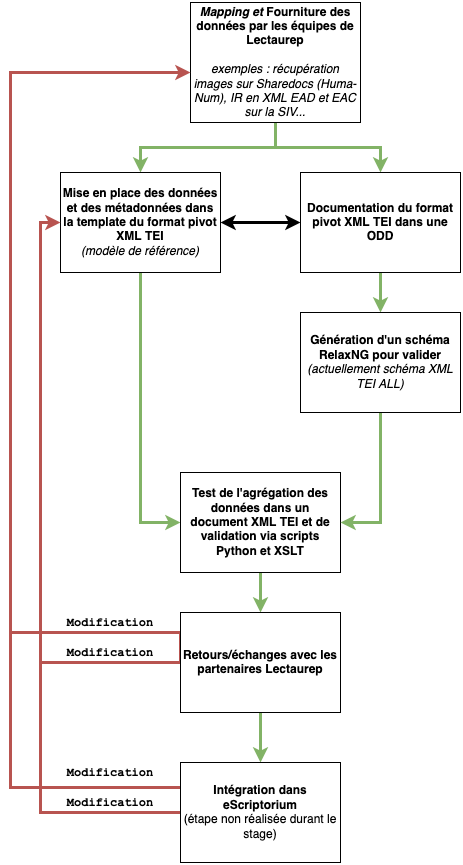
\includegraphics[width=11cm]{workflow_tei_pivot_lectaurep}}}
    \caption{Présentation du workflow pour le format pivot XML TEI Lectaurep mis en place durant le stage  \textcopyright L. Terriel, 2020, Diagrams.net}
    \label{fig:workflow_tei_pivot_lectaurep}
\end{figure}
\clearpage
\thispagestyle{empty}

\chapter{\textit{Workflow} et mise en place d'une première version du fichier pivot XML-TEI}
\section{Un canevas de travail : un fichier XML TEI dans un environnement partagé et ouvert}
Une fois la modélisation des données élaborée et les objectifs du format pivot XML TEI formalisés, il est nécessaire de concevoir le format pivot lui-même. 
Pour résumer et visualiser l'exposition des multiples données Lectaurep dans des champs TEI, il fallait disposer d'un fichier de travail XML suffisamment modulable et ouvert.
Ceci pour synthétiser et inclure les nouvelles réflexions des acteurs qui évoluent au gré des discussions et des réunions concernant la récupération de données spécifiques à Lectaurep. Cela permet l'insertion ou la suppression des nouveaux éléments TEI.\\

On parle alors de mode de développement \inquote{agile} pour la conception du pivot XML TEI. Dès lors, nous avons décidé de travailler dans le cadre d'un canevas (\textit{template}) XML TEI, ou encore un fichier de travail XML-TEI prêt à l'emploi, pour autoriser un grand nombre de modifications à l'intérieur de ce fichier jusqu'à atteindre son état logique, stable et finalisé.\\

% Création de la template
Pour créer la \textit{template} XML-TEI, je suis parti d'un fichier XML-TEI (All) (Cf. Figure \ref{fig:document_minimal_tei}) généré à partir de l'éditeur XML Oxygen. Il s'agit d'une structure minimale (\textit{framework}) en TEI comprenant un élément racine \citecode{<TEI>} ainsi que les deux sous-éléments \citecode{<teiHeader>} et \citecode{<text>}, valide du point de vue d'un schéma Relax NG (REgular LAnguage for XML Next Generation) englobant l'intégralité de la TEI.
   
\begin{figure}[h]
    \centering
    \centerline{\fbox{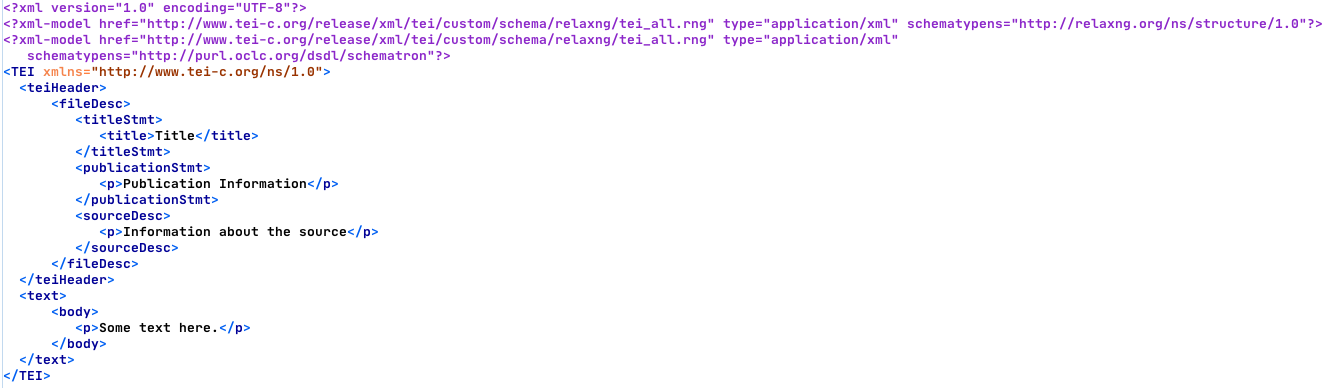
\includegraphics[width=19cm]{document_minimal_tei}}}
    \caption{Document XML-TEI minimal conforme et valide  \textcopyright L. Terriel, 2020, Oxygen XML Editor}
    \label{fig:document_minimal_tei}
\end{figure}

% Environnement de partage de la template
\newpage
Pour mettre en relation et coordonner les membres du projet autour du canevas du format pivot XML-TEI et ainsi prévoir des retours de leurs part, il a été décidé de rendre accessible ce fichier (\citecode{template\_pivot\_TEI\_lectaurep.xml}) via la plate-forme GitLab \footnote{La \textit{template} du format pivot TEI pour Lectaurep est consultable en ligne dans son entier : \url{https://gitlab.inria.fr/almanach/lectaurep/documentation/-/blob/master/Doc/Modélisation_et_schémas_de_validation/template_pivot_TEI_lectaurep.xml} [une permission peut-être demandée] sinon Cf. Annexes,\\ \citecode{/B-Format\_pivot\_XML\_TEI\_Lectaurep/Doc/\\Modélisation\_et\_documentation\_format\_pivot/template\_pivot\_TEI\_lectaurep.xml}} dans le dépôt rassemblant la documentation et les tests effectués à partir de ce format pivot XML TEI.\\

Cet environnement permet de rassembler les suggestions d'améliorations sous la forme de billets que l'on nomment \textit{issues}. Cela permet également d'assurer une traçabilité des évolutions et des versions du format pivot, par le biais des révisions (\textit{commits}) au fil des développements (soit un historique des modifications).\\

Durant le stage, nous avons eu finalement très peu de retours sur le format TEI. Cela peut s'expliquer par le contexte de télé-travail, l'attente de nouvelles fonctionnalités d'\textit{eScriptorium} en priorité et l'outil \textit{GitLab} qui n'est pas encore bien partagé par tous les membres du projet Lectaurep. De plus, certains acteurs ont encore du mal à visualiser l'intégration du fichier XML-TEI dans \textit{eScriptorium}, les premiers tests d'export et d'import en temps voulu dans la plateforme feront surement évoluer ce contexte. 

\section{Une première version du schéma pour le format pivot : repérage des données et choix d'encodage}

\subsection{Repérage des données et règles préalables à l'encodage}

Afin de proposer une première structuration de la \textit{template} du format pivot XML TEI, nous avons décidé, en coordination avec le DMC, de nous concentrer en premier lieu sur le repérage des données (\textit{mapping}\footnote{Nous entendons ici le \textit{data mapping} comme le procédé qui consiste à extraire des données provenant de standards différents, qui seront exposées dans le format pivot XML TEI pour permettre leurs récupération dans d'autres systèmes d'informations.}) et la fourniture des données appartenant aux catégories suivante ( Cf. Table \ref{table:mapping_données_lectaurep} pour le détail des éléments). :  
\bigskip
\begin{itemize}
    \item \textbf{Métadonnées de gestion et de description essentielles} : correspondant aux données extraites des instruments de recherche en XML EAD et EAC fournis par le DMC et disponibles sur la SIV ;
    \item \textbf{Métadonnées techniques des images} : correspondant aux données contenues dans les images, répondant à la spécification EXIF;
    \item \textbf{Images} : essentiellement les noms des fichiers images stockés sur un serveur Humanum (ShareDocs) ;
    \item \textbf{Données provenant des traitements HTR} : correspondent aux transcriptions de vérité terrain (en l'absence de transcriptions HTR), exportées depuis sur la plate-forme eScriptorium, au format XML ALTO.
\end{itemize}
\bigskip
La première mise à plat des données proposée plus haut présente de multiples avantages dans la réalisation du format pivot.\\ 

On relève ainsi : 
\begin{itemize}
    \item la facilité pour accéder aux données dans le temps imparti ;
    \item des problèmes de données redondantes à rassembler ;
    \item une première hiérarchisation (Cf. Figure \ref{fig:oignon_diagram_niveaux_donnees_lectaurep}) des données dans le futur encodage XML TEI, avec trois niveaux bien distincts, allant du plus au degré de granularité (métadonnées liées aux images et aux répertoires de notaires physiques) au plus bas, à savoir le texte de vérité terrain.
\end{itemize}
\begin{figure}
    \centering
    \centerline{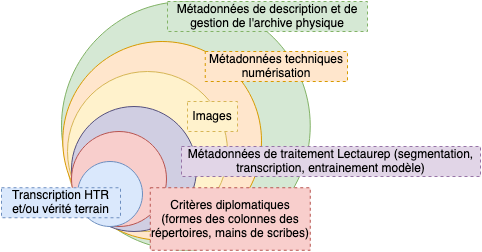
\includegraphics[width=13cm]{oignon_diagram_niveaux_donnees_lectaurep}}
    \caption{Diagramme en oignon des différents niveaux de granularité des données Lectaurep pour représenter les imbrications dans le format pivot XML TEI \textcopyright L. Terriel, 2020, Diagrams.net}
    \label{fig:oignon_diagram_niveaux_donnees_lectaurep}
\end{figure}
\newpage
%---------------------------------
%% TABLEAU : Mapping des principales données Lectaurep utilisées pour la première version du format pivot XML TEI
%% Palette couleur a modifier 
\begin{center}
\begin{longtable}{|p{3cm}|p{2.5cm}|p{5cm}|p{5.5cm}|}
% légende et label du tableau
\caption{\textit{Mapping} des principales données Lectaurep utilisées pour la première version du format pivot XML TEI} 
\label{table:mapping_données_lectaurep}

% ligne de titres du tableau
\\ \hline
\rowcolor[RGB]{220, 220, 220} % gris
\textbf{CATÉGORIES} & \textbf{SCHÉMAS} & \textbf{DONNÉES} & \textbf{ELEMENTS XML} \endhead
        
% gestion du footer        
\hline 
\rowcolor[RGB]{220, 220, 220} \multicolumn{4}{|r|}{{Continue sur la page suivante $\hookrightarrow$}} \\ \hline
\endfoot
\hline \hline
\endlastfoot
        
        % Métadonnées EAD
        \hline
        \rowcolor[RGB]{88, 214, 141} % vert
        \footnotesize{\textbf{Métadonnées de gestion et de description}} & \footnotesize{EAD} & \footnotesize{Noms des fichiers EAD} & \footnotesize{\citecode{<eadid>}} \\
        \cline{3-4}
        \rowcolor[RGB]{88, 214, 141}
        & & \footnotesize{Nom et prénom du notaire} & \footnotesize{\citecode{<persname>}} \\
        \cline{3-4}
        \rowcolor[RGB]{88, 214, 141}
        & & \footnotesize{Étude du notaire} & \footnotesize{\citecode{<corpname>}} \\
        \cline{3-4}
        \rowcolor[RGB]{88, 214, 141}
        & & \footnotesize{Composant pour la description du niveau répertoire} & \footnotesize{\citecode{<c level="series">}} \\
        \cline{3-4}
        \rowcolor[RGB]{88, 214, 141}
        & & \footnotesize{Sous-composant pour la description du niveau minutes} & \footnotesize{\citecode{<c level="recordgrp">}} \\
        \cline{3-4}
        \rowcolor[RGB]{88, 214, 141}
        & & \footnotesize{Cotes des composants et des sous-composants de description} & \footnotesize{\citecode{<unitid type="cote-de-consultation">}} \\
        \cline{3-4}
        \rowcolor[RGB]{88, 214, 141}
        & & \footnotesize{Intitulé des composants et des sous-composants de description} & \footnotesize{\citecode{<unittitle>}} \\
        \cline{3-4}
        \rowcolor[RGB]{88, 214, 141}
        & & \footnotesize{Dates des composants et des sous-composants de description} & \footnotesize{\citecode{<unitdate>}} \\
        \cline{3-4}
        \rowcolor[RGB]{88, 214, 141}
        & & \footnotesize{Description physique des documents compris dans les composants et des sous-composants de description} & \footnotesize{\citecode{<physdesc>}} \\
        \cline{3-4}
        \rowcolor[RGB]{88, 214, 141}
        & & \footnotesize{Informations supplémentaires sur les composants et des sous-composants de description} & \footnotesize{\citecode{<scopecontent>}} \\
        
        % Métadonnées EAC
        \cline{2-4}\rowcolor[RGB]{88, 214, 141}
        & \footnotesize{EAC} & \footnotesize{Dates d'exercices du notaire} & \footnotesize{\citecode{<dateRange>} > \citecode{<fromDate>} / \citecode{<toDate>}}\\
        
        % Métadonnées EXIF
        \hline\rowcolor[RGB]{230, 126, 34} % orange
        \footnotesize{\textbf{Métadonnées techniques des images numérisées}} & \footnotesize{EXIF} & \footnotesize{Titre de la numérisation} & \footnotesize{\citecode{<EXIF:ImageDescription>}} \\
        \cline{3-4}
        \rowcolor[RGB]{230, 126, 34}
        & &  \footnotesize{Version du standard Exif} & \footnotesize{\citecode{<EXIF:ExifVersion>}} \\
        \cline{3-4}
        \rowcolor[RGB]{230, 126, 34}
        & &  \footnotesize{Nom du constructeur de l'équipement} & \footnotesize{\citecode{<EXIF:Make>}} \\
        \cline{3-4}
        \rowcolor[RGB]{230, 126, 34}
        & &  \footnotesize{Nom du modèle de l'équipement} & \footnotesize{\citecode{<EXIF:Model>}} \\
        \cline{3-4}
        \rowcolor[RGB]{230, 126, 34}
        & &  \footnotesize{Orientation de l'image en terme de colonnes et lignes} & \footnotesize{\citecode{<EXIF:Orientation>}} \\
        \cline{3-4}
        \rowcolor[RGB]{230, 126, 34}
        & &  \footnotesize{Nombre de pixels par résolution (\citecode{<EXIF:ResolutionUnit>}) en fonction de la largeur} & \footnotesize{\citecode{<EXIF:XResolution>}} \\
        \cline{3-4}
        \rowcolor[RGB]{230, 126, 34}
        & &  \footnotesize{Nombre de pixels par résolution (\citecode{<EXIF:ResolutionUnit>}) en fonction de la longueur} & \footnotesize{\citecode{<EXIF:YResolution>}} \\
        \cline{3-4}
        \rowcolor[RGB]{230, 126, 34}
        & &  \footnotesize{Unité de mesure de \citecode{<EXIF:XResolution>} et \citecode{<EXIF:YResolution>}} & \footnotesize{\citecode{<EXIF:ResolutionUnit>}} \\
        \cline{3-4}
        \rowcolor[RGB]{230, 126, 34}
        & &  \footnotesize{Date de dernière modification} & \footnotesize{\citecode{<EXIF:ModifyDate>}} \\
        \cline{3-4}
        \rowcolor[RGB]{230, 126, 34}
        & &  \footnotesize{Position des composantes de chrominance par rapport à la composante de luminance. S'applique uniquement aux données compressées de type JPEG. La valeur par défaut est 1} & \footnotesize{\citecode{<EXIF:YCbCrPositioning>}} \\
        \cline{3-4}
        \rowcolor[RGB]{230, 126, 34}
        & &  \footnotesize{Date et heure du stockage de l'image comme donnée numérique} & \footnotesize{\citecode{<EXIF:DateTimeDigitized>}} \\
        \cline{3-4}
        \rowcolor[RGB]{230, 126, 34}
        & &  \footnotesize{Date et heure du stockage de la création de l'image} & \footnotesize{\citecode{<EXIF:DateTime>}} \\
        \cline{3-4}
        \rowcolor[RGB]{230, 126, 34}
        & &  \footnotesize{Informations spécifiques aux données compressées} & \footnotesize{\citecode{<EXIF:ComponentsConfiguration>}} \\
        \cline{3-4}
        \rowcolor[RGB]{230, 126, 34}
        & &  \footnotesize{Si EXIF supporte Flashpix format Ver. 1.0, une valeur par défaut '0100' est inscrite sinon 'NULL'} & \footnotesize{\citecode{<EXIF:FlashpixVersion>}} \\
        \cline{3-4}
        \rowcolor[RGB]{230, 126, 34}
        & &  \footnotesize{Spécifications sur l'espace colorimétrique de l'image} & \footnotesize{\citecode{<EXIF:ColorSpace>}} \\
        
        % Métadonnées ALTO
        \hline\rowcolor[RGB]{52, 152, 219} % bleu
        \footnotesize{\textbf{Données correspondant au document vérité terrain}} & \footnotesize{ALTO} & \footnotesize{Représentation de l'image} & \footnotesize{\citecode{<Layout>}}  \\
        \cline{3-4}
        \rowcolor[RGB]{52, 152, 219}
        & &  \footnotesize{Une page de répertoire} & \footnotesize{\citecode{<Page>}} \\
        \cline{3-4}
        \rowcolor[RGB]{52, 152, 219}
        & &  \footnotesize{Rectangle couvrant la zone imprimée d'une page} & \footnotesize{\citecode{<PrintSpace>}; les coordonnées spatiales de l'élément et les dimensions est donné par les attributs \citecode{@HPOS, @VPOS, @WIDTH, @HEIGHT}} \\
        \cline{3-4}
        \rowcolor[RGB]{52, 152, 219}
        & &  \footnotesize{Bloc de texte qui regroupe les lignes de textes} & \footnotesize{\citecode{<TextBlock>}} \\
        \cline{3-4}
        \rowcolor[RGB]{52, 152, 219}
        & &  \footnotesize{Ligne de texte} & \footnotesize{\citecode{<TextLine>}, elle contient la \textit{baseline} du texte sous la forme de points via l'attribut \citecode{@BASELINE}; les coordonnées spatiales de l'élément et les dimensions est donné par les attributs \citecode{@HPOS, @VPOS, @WIDTH, @HEIGHT}} \\
        \cline{3-4}
        \rowcolor[RGB]{52, 152, 219}
        & &  \footnotesize{Forme de délimitation d'une ligne de texte, si elle n'est pas rectangulaire} & \footnotesize{\citecode{<Shape>}} \\
        \cline{3-4}
        \rowcolor[RGB]{52, 152, 219}
        & &  \footnotesize{Contenu par \citecode{<Shape>}, décrit une forme polygonale} & \footnotesize{\citecode{<Polygon>}, les points sont décrits par l'attribut \citecode{@POINTS}} \\
        \cline{3-4}
        \rowcolor[RGB]{52, 152, 219}
        & &  \footnotesize{Chaîne de caractères de la ligne de texte et leurs positions} & \footnotesize{\citecode{<String>}, les chaînes de caractères de caractères sont comprises dans l'attribut \citecode{@CONTENT}; les coordonnées spatiales de l'élément et les dimensions est donné par les attributs \citecode{@HPOS, @VPOS, @WIDTH, @HEIGHT} identique à \citecode{<TextLine>}} \\
        
\end{longtable}
\end{center}
%---------------------------------
\newpage

% Organisation détaillé et difficultés
L'étape qui suit le repérage des données consistait à répondre à la question : à quel élément TEI faire correspondre un élément $x$ ou $y$ de Lectaurep ?\\ 

Une solution que j'ai retenue consistait à commencer par le haut de l'arbre TEI puis à descendre petit à petit dans l'arborescence en prenant les éléments les uns après les autres. Cependant les éléments de Lectaurep appartenant à trois niveaux de granularités différents, nous devions disposer d'une architecture plus concrète que le canevas \inquote{TEI ALL} principal. Dès lors, j'ai pris le parti d'une  architecture à trois niveaux (Cf. Figure \ref{fig:structure_general_template_tei_lectaurep}) basés sur les trois catégories de données Lectaurep à encoder : 
\begin{itemize}
    \item la balise \citecode{<teiHeader>}\footnote{\cite{tei_tei_nodate}} pour encoder la partie la plus théorique, correspondant aux sources du répertoire c'est-à-dire les métadonnées relatives aux archives physiques et aux images (données issues des fichiers XML EAD/EAC et EXIF), les métadonnées liées à la production du document, les versions du format pivot et des indications sur la publication ;
    \item la balise \citecode{<facsimile>}\footnote{\cite{tei_tei_nodate-2}} pour recevoir les coordonnées (données issues des fichiers XML ALTO) et faire le pont entre les métadonnées générales du \citecode{<teiHeader>} et le \citecode{<text>}, par un système d'identifiants;
    \item la balise \citecode{<body>}\footnote{\cite{tei_tei_nodate-3}} comprise dans la balise \citecode{<text>}\footnote{\cite{tei_tei_nodate-1}} pour accueillir le texte issu du document de vérité terrain, présent dans les fichiers XML ALTO.
\end{itemize}

\begin{figure}[h]
    \centering
    \centerline{\fbox{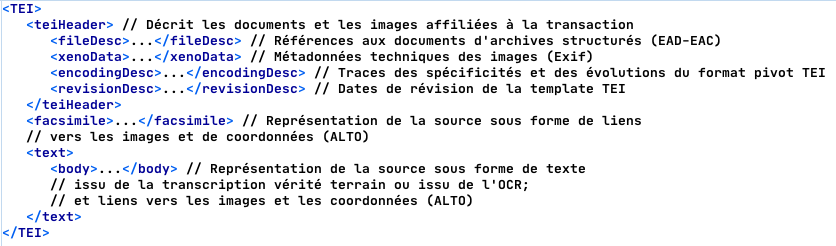
\includegraphics[width=19cm]{structure_general_template_tei_lectaurep}}}
    \caption{Schéma minimal retenu pour l'exposition des données Lectaurep dans un format pivot XML TEI \textcopyright L. Terriel, 2020, Oxygen XML Editor}
    \label{fig:structure_general_template_tei_lectaurep}
\end{figure}
\newpage

\subsection{Encodage des éléments de description des répertoires (EAD et EAC) dans le \citecode{teiHeader}}

Une première approche du \citecode{teiHeader} consiste à modéliser grossièrement les flux entrants et sortants de métadonnées dans cette partie lors d'un import ou d'un export dans eScriptorium, quitte à affiner le travail par la suite (Cf. Figure \ref{fig:flux_teiheader}). La plupart de ces données qui sont visibles dans les IR EAD et NP EAC-CPF trouveront naturellement leurs places dans ces flux.

\begin{figure}[h]
    \centering
    \centerline{\fbox{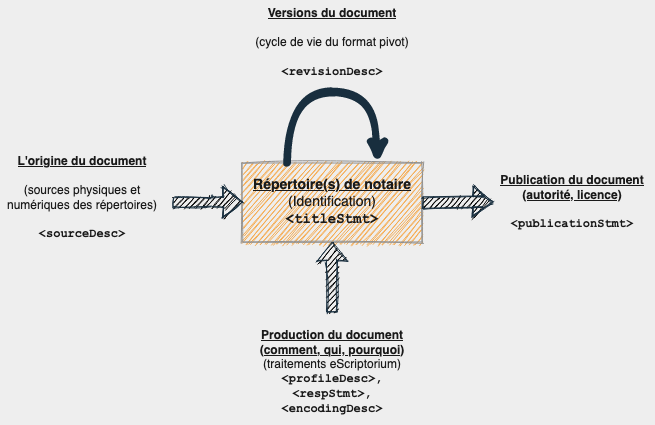
\includegraphics[width=14cm]{flux_teiheader.png}}}
    \caption{Illustration des entrées et des sorties dans le \citecode{teiHeader} \textcopyright L. Terriel, 2020, diagrams.net (inspiré du document fourni par L. Romary, \inquote{The teiHeader at a glance}))}
    \label{fig:flux_teiheader}
\end{figure}

\newpage
En comparant les deux IR \inquote{Images des répertoires du notaire M$^{e}$N} et \inquote{Minutes et répertoires du notaire M$^{e}$N} nous avons pu constater qu'un bon nombre d'informations se croisaient et qu'il était préférable de se baser sur l'IR \inquote{Images des répertoires du notaire M$^{e}$N}, qui contient les informations spécifiques aux répertoires d'un notaire et les liens vers les images de ces derniers plutôt que celui contenant en sus des informations sur les minutes, ce qui aurait complexifié le travail.\\

Pour déterminer quels types d'éléments utiliser dans la conversion EAD vers TEI, nous sommes parti de l'existant et notamment des transformations EAD vers TEI réalisées dans le cadre d'\inquote{HIMANIS}\footnote{\cite{stutzmann_ead-tei_2019}} et du projet \inquote{Enrich}\footnote{\cite{university_of_oxford_-__bodleian_library_ead2enrich_nodate}}. Même si les ambitions d'encodage concernent des documents de natures différentes, certains éléments EAD peuvent être encodés de la même manière en TEI.\\

Dès lors certaines informations comme le nom et le prénom du notaire ont trouvés leurs places dans des éléments \citecode{persName}\footnote{\cite{tei_tei_nodate-9}} (déclinés en \citecode{forename} et \citecode{surname}), le numéro de l'étude à trouvé sa place dans l'élément \citecode{title}\footnote{\cite{tei_tei_nodate-8}} (élément \citecode{corpname} en EAD) et les noms des fichiers d'IR EAD ont quant à eux été reportés dans le \citecode{resp}\footnote{\cite{tei_tei_nodate-7}}.\\

Un certain nombre de valeurs par défaut ont été ajoutées dans le \citecode{publicationStmt}\footnote{\cite{tei_tei_nodate-23}} comme l'organisation de conservation, l'adresse de l'institution etc. Le fait est que ces valeurs ne sont pas censées être modifié au cours du projet.

La réelle difficulté s'est présentée lors de l'encodage des différents niveaux de description EAD des répertoires de notaires et du contenu de ces derniers (Cf. Figure \ref{fig:TEI_EAD_desc_pivot}). Un travail de dépouillement des arbres et de compréhension des logiques d'imbrications de ces IR, souvent complexes, été indispensable. Généralement encodés dans le \citecode{<archDesc>}, il suivent la logique d'imbrications d'un niveau \citecode{<c>}, qui correspond à un répertoire de notaire, qui contient lui-même plusieurs \citecode{<c>} correspondant à des intervalles de pages du répertoire (par exemple l'intervalle des pages 124 r à 150 r\footnote{"r" signifiant "recto".} contiennent une liste chronologique des actes pour la période du 2 janvier au 31 décembre 1877 au 31 décembre 1877). 

\begin{figure}[h!]
  \begin{sideways}
    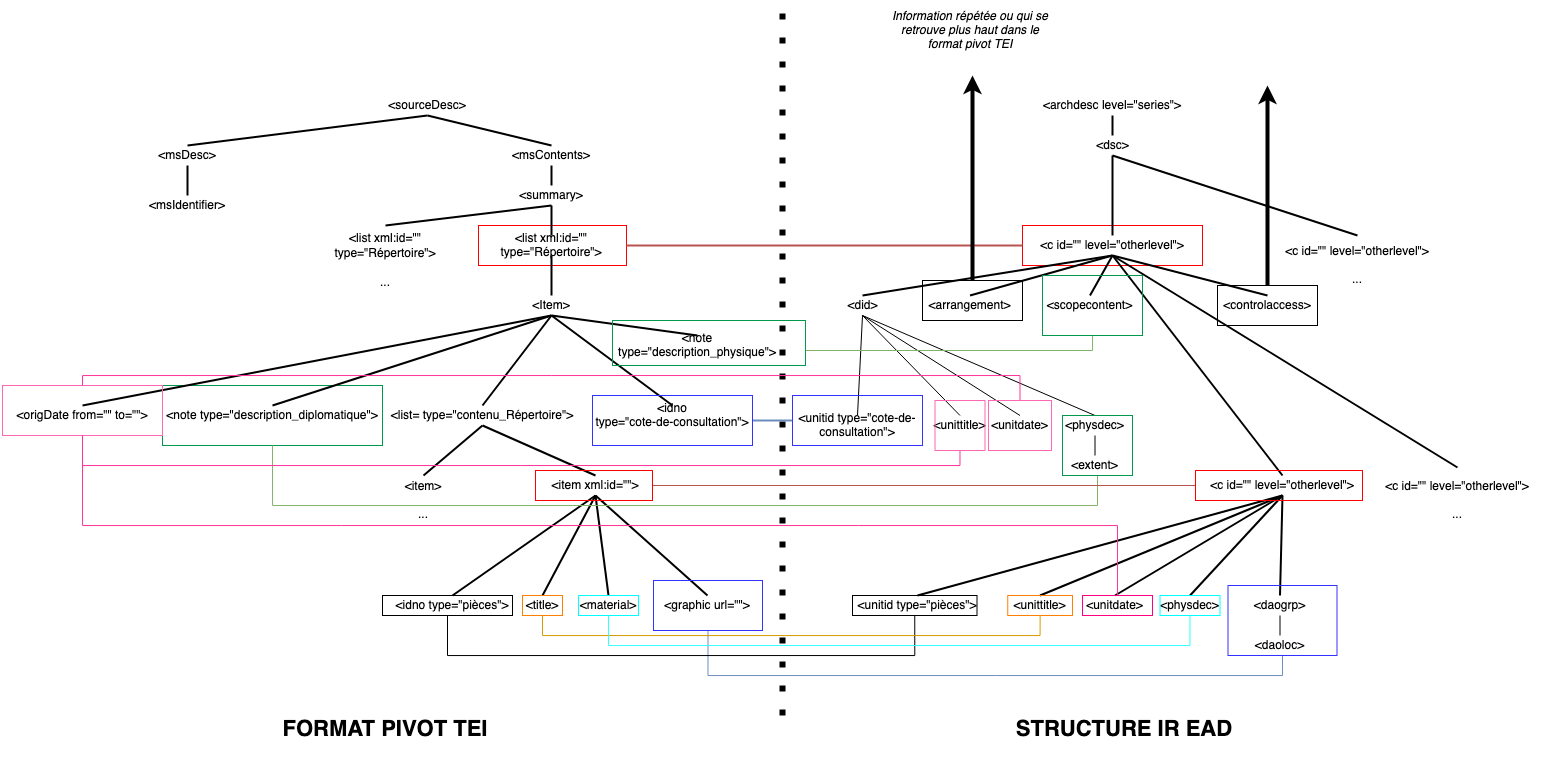
\includegraphics[width=24cm, height=16cm]{TEI_EAD_desc_pivot.png}
  \end{sideways}
  \centering
  \caption{Structure proposée en TEI pour l'encodage des différentes granularités descriptives des éléments EAD \citecode{<c>} pour représenter un répertoire et ses contenus. \textcopyright L.TERRIEL, 2020, Diagrams.net}
  \label{fig:TEI_EAD_desc_pivot}
\end{figure}
\clearpage

Le modèle EAD suit un schéma tel que : le premier niveau de \citecode{<c>}, correspondant au répertoire lui-même, regroupe généralement la cote du répertoire (\citecode{<unitid \\type="cote-de-consultation">}), sa date (\citecode{<unitdate>}), sa description physique (\citecode{<physdesc>}), et des Informations supplémentaires sur les sources (\citecode{<scopecontent>}). 

Les différents niveaux de \citecode{<c>} qui suivent, correspondent au contenu du répertoire. Ils regroupent alors le numéro des pages recto et verso (\citecode{<unitid>}), un titre qui est la liste des actes d'une période donnée (\citecode{<unittitle>}), le nombre de feuillets (\citecode{<unittitle>}), une description optionnelle (\citecode{<scopecontent>}) et une intervalle dans laquelle sont comprises les images numérisées se rapportant aux pages du répertoire (\citecode{<daogrp>} et \citecode{<daoloc>}).\\

À ce moment là, la difficulté fut de savoir si nous choisissons d'encoder un ou des répertoire(s) de notaire(s) lié(s) à une ou des transcription(s) vérité terrain dans le format pivot TEI ?\\

Je suis parti du principe que les utilisatrices ou utilisateurs peuvent effectuer des transcriptions de vérité terrain sur plusieurs répertoires d'un même notaire dans \textit{eScriptorium}. Ainsi, j'ai décidé d'encoder tous les éléments descriptives consécutifs à l'ensemble des répertoires d'un notaire dans le fichier pivot XML-TEI.\\

La structure TEI retenue pour l'encodage des descriptions de répertoire est reportée dans la Figure \ref{fig:TEI_EAD_desc_pivot}. Dans un \citecode{<SourceDesc>}\footnote{\cite{tei_tei_nodate-6}} et un \citecode{<msDesc>}\footnote{\cite{tei_tei_nodate-4}} (permettant de décrire la source de manuscrits), on dispose d'un \citecode{<msIdentifier>}\footnote{\cite{tei_tei_nodate-22}} commun à l'ensemble des répertoires d'un même notaire. Habituellement, réservé à la description d'un manuscrit, le \citecode{<msIdentifier>} fait ici office de carte descriptive unique pour plusieurs répertoires étant donné que les informations sont des valeurs par défaut (pays, lieu, institution, lieu de dépôt) similaires pour les répertoires. On évite donc le phénomène de redondance d'informations. Suit alors le \citecode{<msContents>}\footnote{\cite{tei_tei_nodate-5}} qui rassemble le premier niveau de \citecode{<c>} (EAD) correspondant à un répertoire et les différents niveau de \citecode{<c>} (EAD) imbriqués qui suivent. 

Le premier niveau est alors encodé dans une première liste \citecode{<list>}\footnote{\cite{tei_tei_nodate-21}} portant un \citecode{@type} \inquote{répertoire} et les niveaux inférieurs de \citecode{<c>} sont encodés dans une seconde liste \citecode{<list>} caractérisée par un \citecode{@type} \inquote{contenu\_Répertoire} qui comporte des \citecode{<item>}\footnote{\cite{tei_tei_nodate-20}}  caractérisant les différentes séries de pages pour des périodes d'actes définies. La structure TEI comprise dans les \citecode{<item>} suit ensuite l'ordonnancement logique des descriptions de l'EAD.

\begin{wrapfigure}[20]{l}{11cm}
    \centering
    \centerline{\fbox{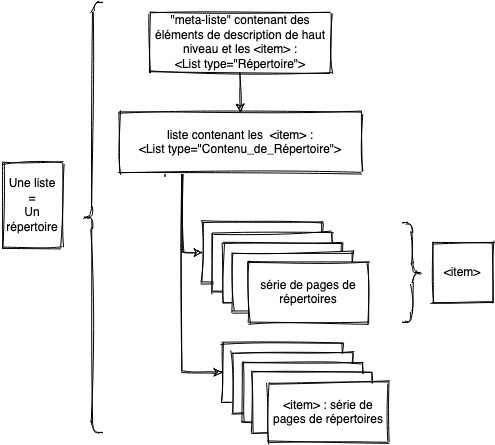
\includegraphics[width=10cm]{metaliste.png}}}
    \caption{Imbrication des deux niveaux de \citecode{<list>} dans le \citecode{<teiHeader>} \textcopyright L. Terriel, 2020, Diagrams.net}
    \label{fig:metaliste}
\end{wrapfigure}

Il y a un décalage à noter : le premier élément \citecode{<list>} (TEI) correspond au premier \citecode{<c>} (EAD) et les éléments \citecode{<item>} de la seconde \citecode{<list>} (TEI) correspondent aux différents \citecode{<c>} (EAD) inférieurs. Dans le format pivot XML-TEI cela se traduit par une premier élément \citecode{<list>} (TEI) portant les métadonnées du répertoire, comme une sorte de \inquote{meta-liste}. (Cf. Figure \ref{fig:metaliste}), et un second élément \citecode{<list>} (TEI) ne faisant que rassembler items compris comme les série de pages de répertoires.\\

Quelques points restent à détailler. La balise EAD \citecode{<arrangement>} n'a pas été prise en compte car elle n'apparaissait pas immédiatement comme un élément indispensable d'encodage pour le projet. Quant à la balise \citecode{<contolaccess>}, répétée à chaque premier niveau de \citecode{<c>}, elle correspond au genre administratif relié à un référentiel des AN. Il nous a paru préférable de rapporter cette information en une seule fois dans une balise TEI \citecode{<additional>}\footnote{\cite{tei_tei_nodate-19}} contenant une balise \citecode{<bibl>}\footnote{\cite{tei_tei_nodate-18}} avec un attribut \citecode{@source}, sur lequel on rapporte le type de référentiel associé. Elle contient elle-même deux balises \citecode{<title>} avec un attribut \citecode{@xml:id}, reliant l'entité du référentiel au format pivot. La balise reçoit alors le titre administratif tel qu'il est décrit dans le référentiel des AN, à savoir \inquote{répertoire d'officier public ministériel}.

Concernant les notices producteurs en EAC-CPF contenant des informations relatives aux notaires (personnes) d'une même étude dans le pviot XML-TEI. 

Dès lors, la stratégie envisagée fût la suivante : dans le \citecode{<msItemStruct>}\footnote{\cite{tei_tei_nodate-17}} nous avons choisi de rapporter un minimum d'informations relatives aux notices producteurs en pointant à l'aide d'attributs \citecode{@source}, placés sur un \citecode{<persName>} pour le notaire et sur un \citecode{<orgName>} pour l'étude. Cet attribut pointe alors directement vers les identifiants des notices producteurs, qui pointent elles mêmes vers d'autres référentiels ainsi que des vocabulaires contrôlés internes aux AN.\\

La conversion de la TEI vers l'EAD a pu poser certaines difficultés majeures. Les différents étages d'imbrication présents dans les IR en EAD des répertoires n'a pas facilité la tâche, et la redondance de certaines informations a obligé un travail souvent fastidieux d'aller-retour entre les deux IR EAD. Il y a fort à parier que la structure envisagée, du fait de sa complexité et de son niveau d'abstraction actuel, évoluera grandement dans la suite du projet. Cependant, cette première structure pose les bases d'une première correspondance entre des éléments des IR et des NP vers la TEI, que les utilisateurs pourraient souhaiter retrouver dans leurs imports et exports d'images dans eScriptorium.

\subsection{Encodage des éléments des métadonnées EXIF dans le \citecode{teiHeader} via des éléments \citecode{xenoData}}

Dans la TEI il n'existe pas d'élément pour décrire la sémantique propre aux métadonnées techniques de numérisation EXIF (Cf. Figure \ref{fig:sortie_exif_metadata}). De plus, il n'est pas conforme aux recommandations de la TEI, d'utiliser un élément existant est de lui spécifier une fonction autre que celle d'origine. Pour donner un exemple d'usages non conforme à la TEI dans ce contexte : \citecode{<item type="EXIF">} ou encore \citecode{<title type="EXIF">}. 

Comme Lou Burnard le souligne, c'est une manière de \inquote{dupliquer} la fonction d'éléments TEI existants\footnote{\cite{burnard_what_2020}}. Pour certains schémas comme le \textit{Dublin Core}, la TEI a anticipé dans son en-tête un certain nombre d'équivalences comme avec le \citecode{<DC:title>} et le \citecode{<title>} TEI. Mais on pourrait envisager dans un projet d'encodage, et cela pour de nombreuses raisons, que l'élément  \citecode{<title>} TEI ne correspond pas assez bien à la sémantique de l'élément DC. On considère alors que l'élément \citecode{<DC:title>} est un élément non-TEI et on souhaiterait une extension pour ce dernier élément, à inclure dans un schéma TEI.\\

Afin d'éviter ces problèmes d'intégrité et de garantir une liberté dans l'encodage, la TEI a prévu l'accueil d'autres vocabulaires XML par un élément \citecode{<xenoData>}\footnote{\cite{tei_tei_nodate-16}}, qui permet d'introduire une extension pour des métadonnées provenant d'un autre schéma.\\

Son fonctionnement est le suivant (Cf. Figure \ref{fig:sortie_exif_xml}) : pour une image, un élément TEI \citecode{<xenoData>} porte dans un attribut \citecode{@xmlns:exif} l'espace de nom (\textit{namespace}) Exif\footnote{Nous avons choisi l'espace de nom EXIF de l'entreprise Adobe, URL : \url{https://github.com/adobe/xmp-docs/blob/master/XMPNamespaces/exif.md} mais il est tout à fait possible d'en utiliser d'autres comme \citecode{http://cipa.jp/exif/1.0/} ou encore \citecode{http://www.w3.org/2003/12/exif/ns}; cependant, il faut faire attention à l'usage des préfixes qui peuvent variés.}. Dès lors, aux niveaux inférieurs, on peut récupérer les différents champs du schéma Exif, en créant des balises précédées d'un préfixe \citecode{exif:}. Un élément \citecode{<exif:Exif>} est requis entre \citecode{<xenoData>} et les métadonnées qui suivent pour permettre la validation du document TEI final.

\begin{figure}[h]
\lstset{language=XML}
\begin{lstlisting}
<xenoData facs="#FRAN_0025_0046_L-0" n="FRAN_0025_0046_L-0.jpg" xmlns:exif="http://ns.adobe.com/exif/1.0/">
   <exif:Exif>
    <exif:ColorSpace>
     65535
    </exif:ColorSpace>
    <exif:DateTimeDigitized>
     2015:09:07 09:33:02
    </exif:DateTimeDigitized>
    <exif:ImageDescription>
     47 - Main frame
    </exif:ImageDescription>
    <exif:Make>
     i2S, Corp.
    </exif:Make>
    <exif:Model>
     SupraScanII [SN: 283910] - Cam7600RGB [SN: 283910]
    </exif:Model>
   </exif:Exif>
  </xenoData>
\end{lstlisting} 
\caption{Un exemple d'encodage d'informations EXIF dans une balise TEI \citecode{<xenoData>}  \textcopyright L. Terriel, 2020, Oxygen XML Editor}
\label{fig:sortie_exif_xml}
\end{figure}
\newpage

\subsection{Encodage des éléments ALTO correspondant aux zones et lignes de texte, et à la transcription dans l'élément \citecode{facsimile} et l'élément \citecode{body}}

L'encodage des fichiers XML ALTO qui contiennent à la fois les coordonnées de polygones (élément ALTO \citecode{<Polygon>}) entourant les zones de texte et de la ligne de base (\citecode{@BASELINE} de l'élément ALTO \citecode{<TextLine>}), ainsi que le texte (attribut \citecode{@CONTENT} de l'élément ALTO \citecode{<String>}) répond à la problématique suivante : comment envisager une structure qui permet de relier le texte à sa représentation spatiale et à l'image ?\\

La mise à plat de l'arbre ALTO a permis de déterminer deux niveaux TEI bien distincts (Cf. Figure \ref{fig:structure_arbre_tei_alto}) : 
\begin{itemize}
    \item une structure \citecode{<facsimile>} contient les représentations des répertoires des notaires sous la forme d'images. Chaque image est encodée dans un élément TEI \citecode{<surface>}\footnote{\cite{tei_tei_nodate-15}} qui constitue une surface en deux dimensions, correspondant à l'image de la page transcrite contenue dans un élément \citecode{<graphic>}\footnote{\cite{tei_tei_nodate-14}}.\\
    Des chercheurs du département de langue allemande et de littérature de l'Université d'Innsbruck en Autriche (qui ont travaillé dans le cadre du projet READ/Transkribus) rappellent que la connexion de l'image de la page avec la transcription n'est pas forcément évidente en TEI. Les méthodes diverges dans la pratique\footnote{\cite{muhlberger_preprint_nodate}, pp.3}, cependant l'élément \citecode{<facsimile>} permet de représenter via des  \citecode{<zone>}\footnote{\cite{tei_tei_nodate-13}} les différents niveaux de représentation ALTO d'un document vérité terrain : \citecode{<PrintSpace>} pour le rectangle couvrant la zone imprimée d'une page, \citecode{<TextBlock>} pour le bloc paragraphe de texte, \citecode{<TextLine>} pour une une ligne de texte, \citecode{<String>} pour contenir les mots et \citecode{<Shape>/<Polygon>} pour la forme du texte, sont reportés dans des attributs \citecode{@type} sur les éléments \citecode{<zone>}.\\
    A noter que les \textit{Guidelines} TEI recommandent l'utilisation d'un élément \citecode{<zone>} plutôt que d'un élément \citecode{<path>}\footnote{\cite{tei_tei_nodate-12}} pour spécifier des lignes comprenant plus de deux points de coordonnées, comme dans le cas des polygones. Les coordonnées spatiales des différents niveaux de représentation de la page sont encodés dans des attributs \citecode{@ulx, @uly, @lrx et @lry} sauf pour l'élément \citecode{<zone>} décrivant le polygone qui utilise un attribut \citecode{@points} spécifique et qui comprend plusieurs valeurs numériques par pairs ($x$,$y$) décrivant les points de la ligne entourant les mots ou les phrases.\\
    \item une structure plus simple comprise dans l'élément TEI \citecode{<body>} de l'élément \citecode{<text>}, permet de récupérer la transcription ALTO. Cette structure s'appuie sur celle proposée par le projet du Dutch Language Institute (INL)\footnote{\cite{dutch_language_institute_alto2tei_nodate}}. La logique est la même que pour le \citecode{<facsimile>} et ces différents niveaux d'imbrications. Cependant la sémantique des balises TEI se concentre sur la représentation de la vérité terrain. Ainsi l'élément \citecode{<div>}\footnote{\cite{tei_tei_nodate-11}} fait référence à la \citecode{<surface>} et contient systématiquement : un élément \citecode{<ab>}\footnote{\cite{tei_tei_nodate-10}} qui correspond à un bloc de texte (\citecode{TextBlock} (ALTO)) contenant un élément \citecode{<w>}\footnote{\cite{tei_tei_nodate-24}} dans lequel on ajoute les données textuelles et un élément \citecode{<lb>}\footnote{\cite{tei_tei_nodate-25}} qui marque le début d'une nouvelle ligne et qui correspond à la (\citecode{TextLine} (ALTO)).
\end{itemize}

\begin{figure}[h!]
    \centering
    \centerline{\fbox{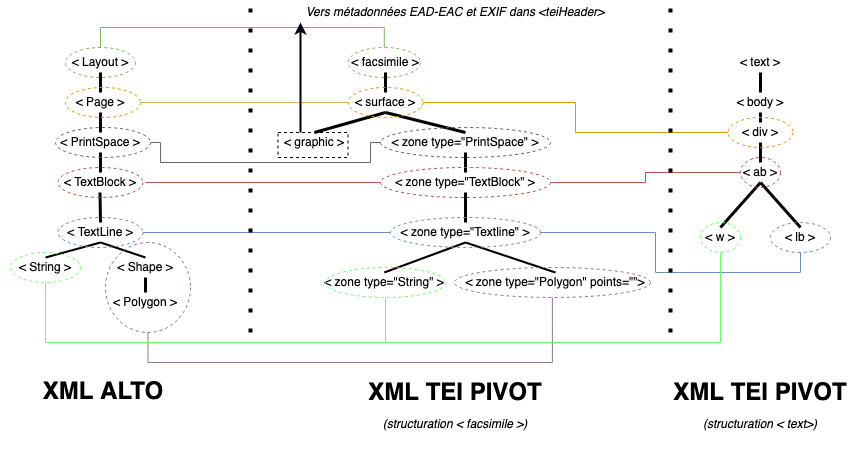
\includegraphics[width=19cm]{Structuration_arbre_alto_tei_liens.png}}}
    \caption{Structure du fichier XML ALTO à gauche et du fichier XML TEI pivot et liens entre les éléments \textcopyright L. Terriel, 2020, Diagrams.net}
    \label{fig:structure_arbre_tei_alto}
\end{figure}
\newpage
Les deux niveaux pour encoder la segmentation et le texte transcrit sont finalement reliés entre eux, mais également à la partie du \citecode{<teiHeader>}, par un système d'identifiants de type \citecode{@url}, \citecode{@facs} et \citecode{@xml:id}.\\

Cette structure à deux niveaux doit encore évoluer dans la suite du projet. En effet les images comprises dans des éléments \citecode{<graphic>} du \citecode{<facsimile>} devront être adaptées pour recevoir les liens du manifeste IIIF (actuellement ce sont les images stockées en local). De plus, la structure du \citecode{<text>} devra encore être modifiées pour accueillir les futures transcriptions HTR (actuellement nous avons traités les vérités terrains), l'étiquetage des entités nommées relevées dans les transcriptions HTR et la structure logique des tableaux des répertoires.
\newpage
\subsection{Compléments sur l'encodage du format pivot XML TEI}

Dans un souci de traçage des modifications ou révisions dans le format pivot et pour spécifier des points particuliers d'encodage dans le format pivot XML-TEI, il nous a paru judicieux de disposer d'un \citecode{<encodingDesc>} suivi d'un 
\citecode{<editorialDecl>} et d'un \citecode{<revisionDesc>} pour y inclure ces informations.

\section{Une ODD pour documenter, partager et valider la canevas XML TEI}

Un format pivot encodé en TEI pour rentrer dans le cadre de l'échange de fichier et être traité par différents systèmes d'informations, doit répondre aux principes de la textit{TEI-conformance}\footnote{\cite{camps_structuration_2017}}, à savoir :
\begin{itemize}
    \item Le document doit respecter les principes du langage XML bien formé;
    \item L'encodage doit pouvoir être validé du point de vue d'un schéma TEI-ALL ou d'un schéma personnalisé qui répond au modèle abstrait de la TEI;
    \item Enfin l'encodage doit être documenté.
\end{itemize}

En effet, le format que nous proposons est en somme une personnalisation de la TEI, pour laquelle il faut rendre compte d'une documentation.

Afin de générer cette documentation nous nous sommes appuyé sur le format de spécification TEI ODD\footnote{TEI, \textit{TEI: Getting Started with P5 ODDs}, URL : \url{https://tei-c.org/guidelines/customization/getting-started-with-p5-odds/}} (\textit{One Document Does it all}) qui permet en outre de :
\begin{itemize}
    \item Générer un schéma RelaxNG ainsi qu'une documentation associée;
    \item Définir les éléments utilisés dans le cadre du format pivot;
    \item Typer les éléments, définir les séquences d'enchaînement des éléments, choisir le type d'attribut à fixer sur les éléments;
    \item s'appuyer sur les macros et les modules de la TEI P5, pour restreindre le nombre d'éléments à utiliser.
\end{itemize}

Pour générer l'ODD spécifique au projet nous avons utilisé une feuille de style \citecode{oddbyexample.xsl} fournie par la TEI, pour générer la documentation à partir du canevas du format pivot XML TEI, à savoir la source \citecode{template\_pivot\_TEI\_lectaurep.xml}, dans les formats suivants : XML (format natif), HTML, pour une visualisation \textit{web}, et PDF\footnote{L'ODD du projet (dans les formats cités) est disponible dans les Annexes, \citecode{/B-Format\_pivot\_XML\_TEI\_Lectaurep/Doc/Modélisation\_et\_documentation\_format\_pivot/}}.

Le format pivot XML-TEI étant en cours de développement, et devant amener encore son lot de modifications, il nous a paru préférable de ne pas rentrer dans le détails des modules TEI. Ceci devant constituer une prochaine étape vers la constitution d'un schéma RelaxNG propre au projet, celui-ci étant toujours le schéma TEI-ALL.\\ 

Cette \inquote{ODD de travail} rappelle les objectifs actuels, rend visible le canevas de la présente version du format pivot (pour les personnes ne disposant pas d'un éditeur XML, par exemple), de suggérer des axes de travail pour la suite, enfin de rendre accessible la documentation sur les éléments utilisées. L'ODD fournie au format HTML, pourrait tout à fait être partagée sur le blog \textit{hypothèses} Lectaurep dans le cadre d'une diffusion des savoirs-faire et dans la logique de retours d'expériences.

\section{Les évolutions du format pivot XML-TEI pour la suite du projet}

Pour la suite à donner au format pivot XML TEI, les cas suivants ont pu envisagés :
\begin{itemize}
    \item Trouver le moyen d'intégrer les liens vers les manifestes IIIF et les URI vers les images dans les éléments TEI \citecode{<graphic>}, plutôt que d'utiliser les images stockées globalement, pour tester leurs récupération;\\
    \item Envisager une structure d'accueil TEI pour les futures transcriptions TEI;\\
    \item Proposer un balisage pour les entités nommées dans la future transcription HTR en se basant sur les éléments TEI au niveau de la balise \citecode{<body>} afin d'étiqueter les personnes (\citecode{<person>}), les prix (\citecode{<num type="prix\_acte">}), lieux (\citecode{<placeName>}), les dates (\citecode{<date>}), les professions (\citecode{<roleName type="metier">}), les titres honorifiques (\citecode{<roleName type="honorifique">}) etc. Là encore tout dépend du niveau d'information que l'on souhaite récupérer et des choix de balises qui seront faits\footnote{\cite{le_pevedic_retour_2016}};\\
    \item Le format pivot XML TEI devra faire ressortir, à terme les logiques de structures internes des colonnes du tableaux des répertoires, notamment pour développer des éditions \inquote{paléographique}. Sur ce dernier point, Laurent Romary, directeur de recherche pour INRIA et qui a suivi la constitution du format pivot XML TEI, a suggéré, dans un premier temps, de rendre compte de la sémantique des colonnes du tableau des répertoires (ce sur quoi travaille actuellement eScriptorium). 
    
    Par exemple, une colonne correspond au type d'acte, la suivante au prix, la suivante au client etc.; et dans un deuxième temps, il faudrait réunir les blocs horizontaux similaires si ces blocs concernent un même acte. Le dernier point ne constitue pas une tâche évidente dans la mesure où les répertoires de notaires présentent des écritures pouvant parfois déborder des colonnes ou prendre de la place sur plusieurs lignes. Toujours est-il que des outils existent comme Grobid\footnote{Grobid documentation, URL: \url{https://grobid.readthedocs.io/en/latest/Introduction/}} (\textit{GeneRation Of BIbliographic Data}), toujours en développement, pour extraire des informations sur la structure d'un document, parser et restructurer ces informations dans un format XML-TEI;\\
    \item Approfondir les logiques d'écritures propres au XIX$^e$ siècle : il serait envisageable de relier certains éléments de mise en forme du texte dans le répertoire à un référentiel de mains générique spécifique et caractéristique des répertoires de notaires dans le \citecode{<msDesc>} contenant des éléments \citecode{<handDesc>};\\
    \item Dans une logique d'entonnoir, au fur et à mesure de l'avancement des choix de balisages, il faudra formaliser ces règles dans l'ODD afin de restreindre les modules TEI pour générer un schéma RelaxNG propre au projet;\\
    \item Effectuer des tests d'intégration du format pivot XML TEI dans la plate-forme eScriptorium pour permettre des retours et d'envisager d'autres possibilités. 
\end{itemize}
\newpage
\section{Simuler l'agrégation des données et la validation d'un fichier XML TEI via un \textit{script} Python}\label{generator-lecto-dev}

Certains acteurs du projet Lectaurep ressentaient le besoin de visualiser les données provenant des sources XML EAD-EAC, ALTO et des images dans la première version du canevas XML-TEI.\\

Cependant, un encodage \inquote{à la main} des données, une à une dans un fichier XML-TEI était impensable pour de nombreux fichiers. Pour réaliser cette tâche, la création d'un script informatique pour permettre le traitement automatique afin d'extraire les informations des fichiers, les structurer dans l'arborescence TEI souhaitée et valider cette arborescence par le biais d'un schéma de validation.\\

J'ai donc réalisé un outil, sous la forme d'un CLI (\textit{Command Line Interface}) appelé \textit{Generator Lectaurep-TEI}, basé sur des scripts en langage Python pour mener à bien cette tâche. Parmi ces scripts, un script d'exécution principal \citecode{main.py} chargé de dérouler les différentes étapes du programme, une série de trois scripts asservis au script principal conçu comme des modules : \citecode{build\_utils.py}, \citecode{extract\_utils.py}, et \citecode{validation\_utils.py} contenant des fonctions utiles pour réaliser des tâches précises durant le processus de traitement des fichiers ainsi que deux feuilles de transformation rédigées en XSLT : \citecode{Lectaurep\_ALTO2TEI.xsl} et \citecode{Lectaurep\_EADEAC2TEI.xsl}.\\ L'objectif étant de parser et de restructurer les fichiers XML en entrée pour récupérer les informations dans une arborescence TEI en sortie. Nous reviendrons sur ces feuilles de styles dans la section suivante.\footnote{Le programme composé des scripts, des feuilles de transformation XSL, des fichiers de tests, des schémas de validation, et d'une documentation d'installation et de fonctionnement \inquote{lisez-moi} (\citecode{readme.md}) est disponible dans l'Annexe B, \\
\citecode{/B-Format\_pivot\_XML\_TEI\_Lectaurep/Generator\_Lectaurep2TEI}}.\\

Afin de tester le programme nous avons formé un jeu de données autour des fichiers de répertoires du notaire Legay (\citecode{Set\_test\_Legay}). Ce set de données est constitué d'un dossier \citecode{Data\_xml\_alto} qui contient les fichiers XML ALTO, d'un autre contenant les fichiers XML EAD-EAC :  \citecode{Data\_xml\_ead\\\_eac} et enfin d'un dossier \citecode{images} rassemblant les images de répertoires. Il s'agit là de la configuration de fichiers dont les utilisateurs doivent disposer.\\
\newpage
Pour fonctionner, les scripts nécessitent un environnement virtuel basé sur Python 3 et dans lequel seront installés :

\begin{itemize}
    \item \textbf{lxml} (version 4.5) : il permet de manipuler des fichiers XML et HTML. Il est utilisé ici pour son module de fonctions pour lire des schémas de validation (DTD, RelaxNG, XMLSchema, Schematron);
    \item \textbf{beautifulsoup4} (version 4.4) : autre parseur de fichiers HTML et XML. Il est utilisé pour sa fonction de manipulation des arbres XML;
    \item \textbf{pyfiglet} (version 0.8.0), \textbf{tqdm} (version 4.46.1) et \textbf{termcolor} (version 1.1.0) : une série de \textit{packages} utilisés pour obtenir un visuel spécifique (couleur des messages, barres d'avancement etc.) sur la progression des tâches.
\end{itemize}
\bigskip
Les autres \textit{packages} sont déjà inclus dans la distribution Python (modules et fonctions \textit{built-in}). Tous ces \textit{packages} Python sont listés dans le fichier \citecode{requirements.txt} pour faciliter l'installation. Une documentation qui résume les étapes d'installation ainsi que les étapes d'installations sont disponibles dans un fichier de type \inquote{lisez-moi} (\citecode{readme.md}).\\

\subsection{Les différentes étapes du programme : le script principal \citecode{main.py}}

Avant de concevoir le programme j'ai modélisé un algorithme afin de diviser les tâches de travail et de résumer chaque étape du programme permettant d'accélérer considérablement le développement de l'outil (Cf. Figure \ref{fig:generateur_tei}).\\

Le programme réalise les étapes suivantes :
\begin{enumerate}
    \item L'usager entre une ligne de commande pour indiquer l'emplacement des différents fichiers. Chacun de ces chemins est renseigné par grâce à un préfixe (\textbf{- -images}, \textbf{- -ead\_eac}, \textbf{- -alto}, \textbf{- -rng)}. L'usager donne également un nom au fichier XML qu'il souhaite obtenir en sortie, préfixé (\textbf{- -output)};
    \item Le script principal charge et stocke distinctement les différents fichiers à partir de l'extension de ces derniers (le script fait un appel au module \citecode{extract\_utils.py} via le \textit{package built-in} \textit{glob} qui gère la recherche de chemins de style Unix);
    \item Une étape préliminaire contrôle la présence des fichiers, en cas d'absence de ces derniers le programme envoie un message (\textit{log}) d'erreur et interrompt le programme en cours;
    \item La première étape du traitement consiste à créer des fichiers XML qui sont des catalogues qui regroupent les fichiers XML fournis en entrée (module \citecode{build\_utils.py}). Les fichiers XML ALTO sont disposés dans un premier catalogue XML (\citecode{catalog\_alto.xml}) et les fichiers XML EAD-EAC suivent la même procédure (\citecode{catalog\_ead\_eac.xml}). Nous verrons dans la section suivantes plus en détail l'utilité de ces catalogues XML pour les transformation XSLT;
    \item L'étape suivante consiste à extraire des fichiers, dans les catalogues XML. Les données sont placées dans deux nouvelles arborescence XML distinctes qui correspondent aux informations des fichiers XML ALTO placés eux dans une première structure arborescente réparti sur deux niveaux : \citecode{<facsimile>} et \citecode{<text>}. Les informations des XML ALTO sont disposés dans un \citecode{<teiHeader>} dans une seconde structure arborescente. Les structures sont créés à partir des feuilles XSL, qui sont lues par le pré-processeur XSL java Saxon. Ce dernier est appelé par une ligne de commande qui s'exécute automatiquement durant le programme par l'intermédiaire d'une fonction du \textit{package} OS qui permet d'interagir avec le système d'exploitation;
    \item Les deux structures sont alors rassemblées (\textit{merge}) en une seule qui comprend désormais le \citecode{<teiHeader>}, le \citecode{<facsimile>} et le \citecode{<text>};
    \item Les métadonnées EXIF sont extraites des images et rassemblées dans une arborescence \citecode{<xenoData>} qui rejoint l'arborescence précédente, de manière à constituer le fichier XML TEI complet. À noter que durant cette étape certaines valeurs EXIF n'ont pas été décodées au moment de leurs insertions dans l'arborescence. Nous avons donc ajouté une valeur par défaut \inquote{bytes values}, pour celles qui ne sont pas prises en compte\footnote{Une balise \citecode{<exif>} doit obligatoirement contenir une valeur. Dans le canevas XML TEI j'ai ajouté au niveau du \citecode{<encodingDesc>} cette information de manière à ce que l'on puisse l'interpréter ultérieurement.};
    \item Le programme génère alors une sortie XML comme étant le nouveau fichier XML TEI et le sauvegarde dans le dossier par défaut 
    \citecode{Output};
    \item Si l'usager à spécifié une option de validation (\textbf{- -rng}) et renseigné un schéma de validation, le programme appelle le module \citecode{validation\_utils.py} qui vérifie la conformité XML et la validation du XML TEI\footnote{Pendant les tests nous avons utilisé un schéma RelaxNG TEI ALL.}. Le programme s'interrompt après avoir renvoyé un message d'erreur ou de succès à l'usager.
\end{enumerate}
\begin{figure}[H]
    \centering
    \centerline{\fbox{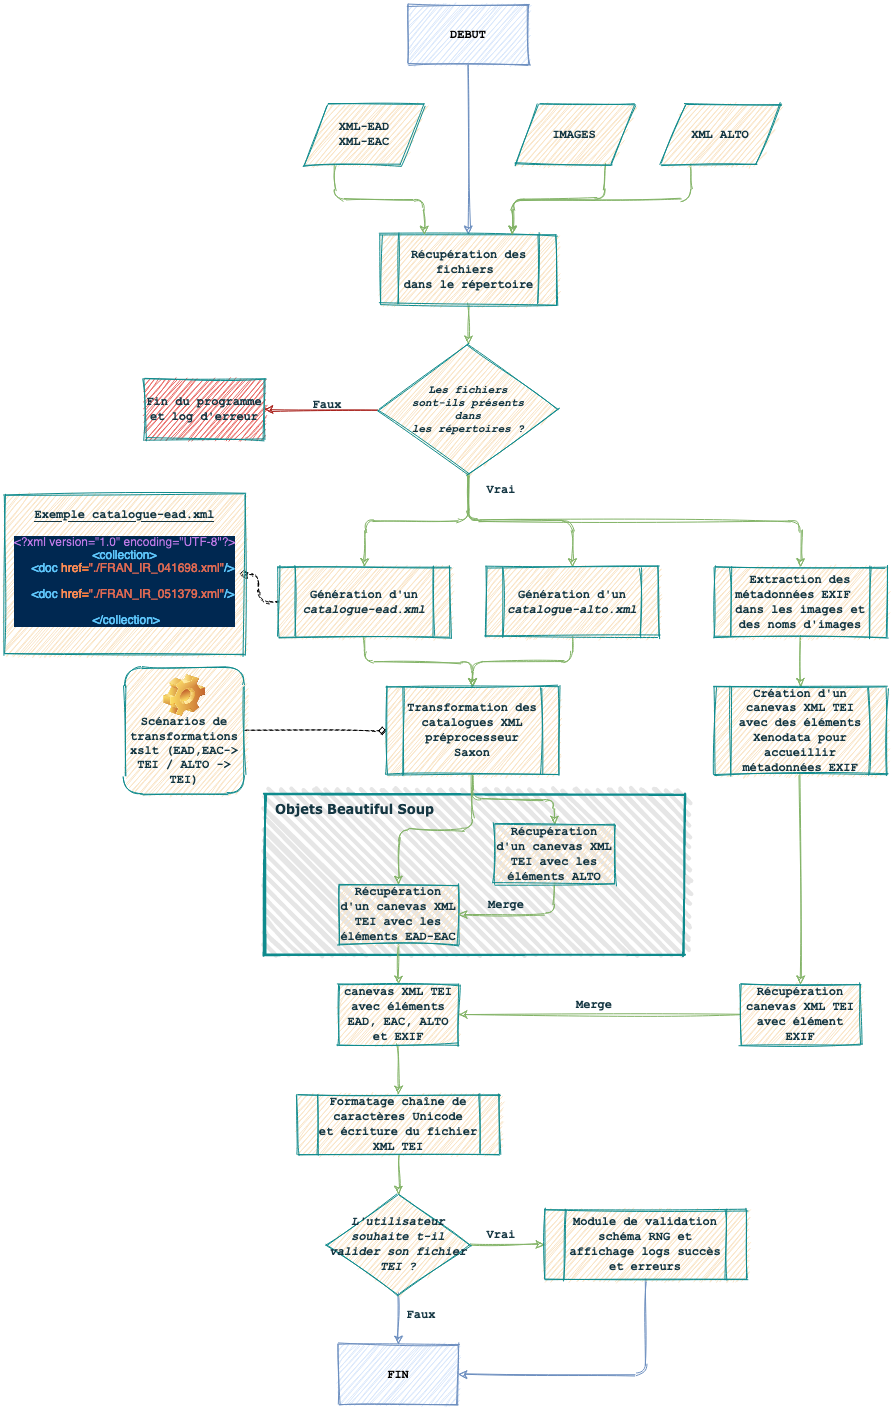
\includegraphics[width=17cm, height=22.5cm]{Générateur-XML-TEI.png}}}
    \caption{Algorigramme du programme Generator Lectaurep-TEI pour simuler la visualisation d'un format XML TEI pivot comprenant des données provenant de fichiers XML ALTO, EAD et EAC-CPF et des métadonnées EXIF provenant d'images.   \textcopyright L. Terriel, 2020, Diagrams.net}
    \label{fig:generateur_tei}
\end{figure}
\begin{figure}[h]
    \centering
    \centerline{\fbox{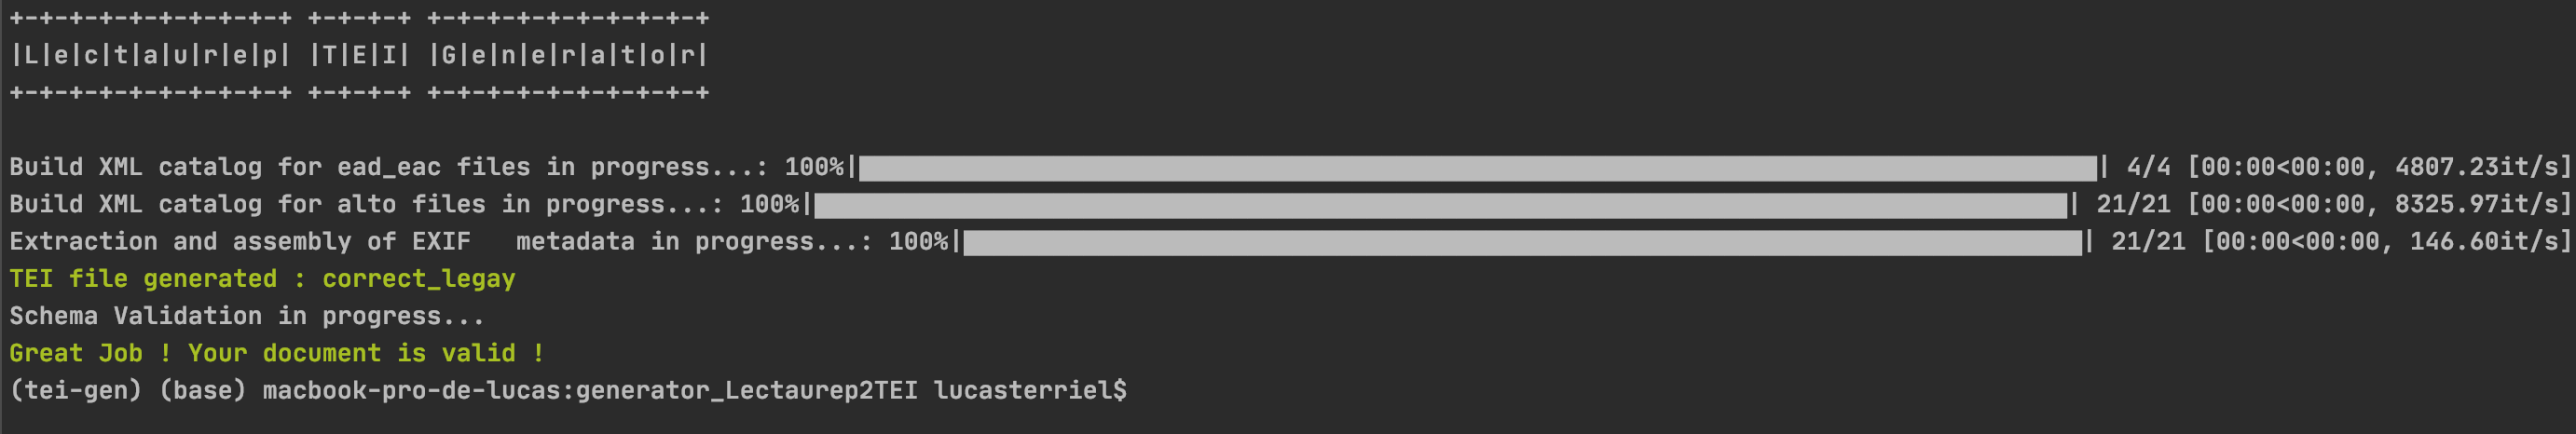
\includegraphics[width=19cm]{generator-lec-tei-prompt.png}}}
    \caption{Capture du terminal qui montre le bon déroulement du CLI Generator Lectaurep-TEI.   \textcopyright L. Terriel, 2020, Diagrams.net}
    \label{fig:prompt-lec-tei}
\end{figure}

\subsection{Deux feuilles de styles XSLT pour obtenir des arborescences TEI : \citecode{Lectaurep\_ALTO2TEI.xsl} et \citecode{Lectaurep\_EADEAC2TEI.xsl}}

Nous avons esquissé, plus haut, durant l'exécution du programme le rôle des feuilles de transformation XSL : \citecode{Lectaurep\_ALTO2TEI.xsl} et \citecode{Lectaurep\_EADEAC2TEI.xsl}. Pour rappel une transformation XSL se base sur le langage XSLT qui est une syntaxe XML permettant de spécifier, suivant des règles de transformation, de quelle manière un ou des fichier(s) XML doivent être transformé(s) en un autre document (Cf. Figure \ref{fig:example_XSLT}). Il s'agit en somme d'un langage de réecriture d'arbres. Une transformation s'effectue à l'aide d'un pré-processeur (comme Saxon ou Xalan écrits tous les deux en langage Java) et peut s'exécuter dans un éditeur XML comme \textit{Oxygen XML Editor} ou bien en ligne de commande comme dans le programme Generator Lectaurep-TEI.\\

\begin{figure}[h!]
    \centering
    \centerline{\fbox{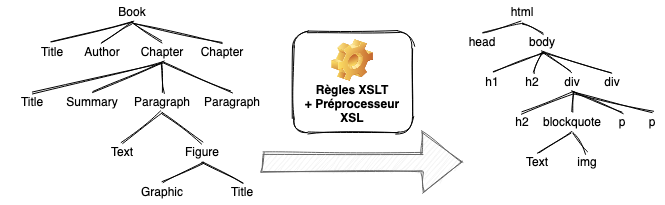
\includegraphics[width=15cm]{exemple_XSLT.png}}}
    \caption{Illustration d'une transformation XSLT d'un document XML vers un document HTML  \textcopyright L. Terriel, 2020, Diagrams.net}
    \label{fig:example_XSLT}
\end{figure}
\newpage
Les feuilles de style créées pour le programme sont les suivantes : 
\begin{itemize}
    \item \citecode{Lectaurep\_ALTO2TEI.xsl} : cette feuille XSL correspond à la transformation des fichiers XML ALTO vers des structures TEI \citecode{<facsimile>} et \citecode{<text>}. Ce fichier a été repris et adapté sur la base de la feuille XSL proposée par le Dutch Language Institute (INL)\footnote{\cite{dutch_language_institute_alto2tei_nodate}}. Certaines règles de transformation ont dû être modifiées pour correspondre aux balises spécifiques des fichiers XML ALTO de Lectaurep. De plus, une fonction XSLT a dû être implémentée en sus pour permettre de concaténer les points de coordonnées de l'élément ALTO \citecode{<Polygon>} sous la forme de coordonnées avec un séparateur ($x$,$y$ $x$,$y$ $x$,$y$ ...)  pour être inclus dans l'attribut \citecode{@points} de l'élément TEI \citecode{<zone type="Polygon">}\footnote{suivre l'échange du 24 août 2020 sur \textit{stackoverflow}, URL : \url{https://stackoverflow.com/questions/63569657/xslt-concatenate-a-list-of-numbers-with-a-separator-according-to-a-pattern}}, sans cela le document TEI ne pouvait être validé.\\ 
    \item \citecode{Lectaurep\_EADEAC2TEI.xsl} : cette feuille XSL correspond à la transformation des éléments XML EAD-EAC vers une structure \citecode{<teiHeader>}. Elle a été créée \textit{ex-nihilo} pour correspondre à la structure d'acceuil présenté dans le canevas XML-TEI de Lectaurep.  
\end{itemize}
\bigskip
Ces feuilles XSL s'appliquent à de très nombreux fichiers en même temps (4 fichiers XML EAD-EAC et 21 fichiers XML ALTO pour les tests). Dès lors j'ai dû trouver un moyen de parcourir l'ensemble de ces fichiers en une seule fois pour en extraire les informations vers le nouveau document TEI. Une astuce consiste à recourir à la fonction XPath\footnote{\textbf{XPath} est un langage de requête utilisé pour parcourir ou localiser une portion d'un document XML. XSLT utilise XPath dans ces règles pour repérer des éléments à modifier.} \citecode{collection()} dans les feuilles XSL\footnote{Pour plus de précision sur l'utilisation de la fonction XPath \citecode{collection()} consulter \cite{holmes_xpath_nodate-1}}. Son utilisation requiert alors de constituer au préalable un catalogue regroupant les fichiers XML à transformer (Cf. Figure \ref{fig:catalogue}). La fonction est placé dans la feuille XSL avec le nom du fichier XML \inquote{catalogue} à transformer. 

À partir de là, les règles de transformation seront effectives sur l'ensemble des documents XML contenus dans ce catalogue et présentant le sous-ensemble localisé par la requête XPath.

\begin{figure}[h!]
\lstset{language=XML}
\begin{lstlisting}
<collection>
 <doc href="./FRAN_IR_051379.xml"/>
 <doc href="./FRAN_NP_011490.xml"/>
 <doc href="./FRAN_IR_041698.xml"/>
 <doc href="./FRAN_NP_010150.xml"/>
</collection>
\end{lstlisting}
\caption{Exemple d'un fichier XML \inquote{catalogue} qui regroupe des fichiers XML EAD-EAC  \textcopyright L. Terriel, 2020}
\label{fig:catalogue}
\end{figure}
\newpage
\subsection{Perspectives d'évolution pour le \textit{Generator Lectaurep-TEI}}

Il n'a pas été prévu, pour le moment, d'apporter des modifications majeures à l'outil. En effet, celui-ci suit de près les évolutions du canevas XML-TEI dans la continuité du projet. Quand le schéma et les réflexions de Lectaurep autour du canevas seront plus développés, il serait envisageable, grâce à ce petit programme de générer un fichier XML-TEI et de tester son intégration dans eScriptorium ou dans des applications de récupération de données plus spécifiques. Cependant, les différents modules développés pour ce script, comme le validateur RelaxNG (\citecode{validation\_utils.py}) ainsi que les feuilles de transformation XSL peuvent être réutilisées indépendamment de l'outil dans d'autres types de projets par ALMAnaCH.
\clearpage
\thispagestyle{empty}